\chapter{Dielectron Analysis Details}
\label{chap:analysis}

\section{Event Selection and Centrality Definition}
\label{centrality}
The data set used in this analysis is from U + U collisions at $\sqrt{s_{NN}}$ = 193 GeV in RHIC run year 2012 (Run12). The minimum-bias (MB) trigger is defined as a coincidence between the two VPDs, a coincidence between the two ZDCs, and an online collision vertex cut. Moreover, a pile-up protection at the trigger level was applied for the data taking.

Events used in this analysis are required to have a valid collision vertex (primary vertex) within 30 cm of the TPC center along $z$ direction (the direction along beam axis) to ensure uniform a TPC acceptance. Furthermore, the distance between the collision vertex along $z$ direction constructed by the TPC ($V_{z}^{TPC}$) and the VPD ($V_{z}^{VPD}$, fast detector) is within 3 cm to reject the event with wrong reconstructed TPC vertex from different bunch-crossing collisions. To reject the events from the beam hitting the beam pipe, vertex with a radial length less than 2 cm with respect to the beam pipe center is required. After event selection, 270 million minimum-bias events are finally used in this analysis. Table~\ref{eventselection} lists the event selection criteria.

\begin{table}[htp]
\centering
\caption{Event selection in U + U collisions at 193 GeV.}
\label{eventselection}
\begin{tabular}{c}
\toprule[1.6pt]
Event Selection Criteria \\
\midrule[1.2pt]
\multirow{2}*{$|V_{r}|<$ 2 cm} \\
\\
\multirow{2}*{$|V_{z}^{TPC}|<$ 30 cm} \\
\\
\multirow{2}*{$|V_{z}^{TPC} - V_{z}^{VPD}|<$ 3cm} \\ 
\\  
\bottomrule[1.6pt]
\end{tabular}
\end{table}

The centrality in U + U collisions at 193 GeV is defined using the uncorrected charged particle density ($dN_{ch}/dy$). The primary tracks with $|\eta|$ $\leq$ 0.5, dca $\leq$ 3 cm and nHitsFit $\geq$ 10 (number of hits used for track fitting) are used to calculate the $dN_{ch}/dy$. Furthermore, the $dN_{ch}/dy$ is corrected for the $V_{z}^{TPC}$ and luminosity dependence to account for the acceptance and efficiency changes on the measured $dN_{ch}/dy$. Then the $dN_{ch}/dy$ is compared to a Monte Carlo (MC) Glauber calculation~\cite{MCGlauber} to delineate the centrality bins, the equivalent number of binary nucleon + nucleon collisions ($N_{bin}$ or $N_{coll}$) and the number of participants ($N_{part}$) for nucleus + nucleus collisions. Table~\ref{centrality} lists the $\langle$$N_{coll}$$\rangle$ and $\langle$$N_{part}$$\rangle$ from Glauber model for each defined centrality bin in U + U collisions at $\sqrt{s_{NN}}$ = 193 GeV. The 0-80\% and finer centrality-bins within this range are used in this analysis, because the 80-100\% centrality has significant trigger bias due to vertex inefficiency at low charged particle density.  

\begin{table}[htp]
\centering
\caption{Centrality bins and corresponding $\langle$$N_{coll}$$\rangle$, $\langle$$N_{part}$$\rangle$ in U + U at 193 GeV.}
\label{centrality}
\newcolumntype{V}{!{\vrule width 1.6pt}}
\begin{tabular}{Vc|r@{.}l|r@{.}lVc|r@{.}l|r@{.}lV}
\Xhline{1.6pt}
Centrality & \multicolumn{2}{c|}{$\langle$$N_{coll}$$\rangle$} & \multicolumn{2}{cV}{$\langle$$N_{part}$$\rangle$} & Centrality & \multicolumn{2}{c|}{$\langle$$N_{coll}$$\rangle$} & \multicolumn{2}{cV}{$\langle$$N_{part}$$\rangle$} \\
\Xhline{1.2pt}
0-5\% & 1281&26 & 414&87 & 5-10\% & 1010&97 & 355&42 \\ \hline
10-15\% & 798&53 & 300&92 & 15-20\% & 628&01 & 253&66 \\ \hline
20-25\% & 490&60 & 212&84 & 25-30\% & 379&86 & 177&48 \\ \hline
30-35\% & 290&31 & 146&78 & 35-40\% & 217&35 & 119&63 \\ \hline
40-45\% & 160&03 & 96&34 & 45-50\% & 115&69 & 76&43 \\ \hline
50-55\% & 81&76 & 59&55 & 55-60\% & 56&98 & 45&73 \\ \hline
60-65\% & 38&36 & 34&01 & 65-70\% & 25&06 & 24&55 \\ \hline
70-75\% & 16&28 & 17&46 & 75-80\% & 10&23 & 11&98 \\ \hline
\Xhline{1.6pt}
\end{tabular}
\end{table}

\section{Electron Identification}

\subsection{Track Selection}
The interested electrons (including positrons if not specified) are mainly from the collision point or short-lived particle decays close to the collision point. Thus the primary tracks, including the primary vertex for the track fitting resulting in a better momentum resolution, are used in this analysis. The primary tracks are required to satisfy the following selection criteria: $p_{T}$ is $\geq$ 0.2 GeV/$c$ to ensure that the track can pass through the TPC; the Distance of Closest Approach (dca) to the primary vertex is $\leq$ 1 cm to reduce contributions from secondary decays; the number of hit points (nHitsFit) along the track is $\geq$ 20 (of a maximum of 45) to ensure good momentum resolution; the ratio of number of hit points along the track over the number of maximum possible points (nHitsPoss) is $\geq$ 0.52 to suppress the possibility of selecting duplicated short tracks from track splitting; the number of points used for calculating $\langle$$dE/dx$$\rangle$ (nHitsDedx) is $\geq$ 15 to ensure good $dE/dx$ resolution; at last, the track is required to match with the TOF and restricted to $|\eta|$ $\leq$ 1.
 
\subsection{Electron Identification Cuts}

The electron candidates could be identified by combining the TPC and TOF. The TPC provides particle identification utilizing the $dE/dx$, because different particle species with the same momentum may have different $dE/dx$. However, in some momentum regions, the TPC can not identify different particle species with very similar $dE/dx$ (e.g. $e/K$ at p $\approx$ 0.5 GeV/$c$, $e/p$ at p $\approx$ 1 GeV/$c$). Different particle species with the same momentum have different velocities, thus the TOF with $<$80 ps time resolution can be used to identify different particle species in the $dE/dx$ crossover regions by precise velocity information ($1/\beta$ = $ct/l$). The normalized $dE/dx$, defined in Eq.~\ref{nsigmae:eq}, instead of $dE/dx$ is used in this analysis. Where $\langle{dE/dx}\rangle^{Mea.}$ and $\langle{dE/dx}\rangle^{Th.}_{e}$ represent measured and theoretical $dE/dx$, and $R_{dE/dx}$ is the STAR TPC $dE/dx$ resolution (typically $\sim$8\%). If the $dE/dx$ (truncated $dE/dx$) calibration is done perfectly, the $n\sigma_{e}$ of electron sample should be close to a standard Gaussian distribution (mean $=$ 0, $\sigma = $ 1).
\begin{equation}
n\sigma_e = \frac{1}{R_{dE/dx}}log\frac{\langle{dE/dx}\rangle^{Mea.}}{\langle{dE/dx}\rangle^{Th.}_{e}}
\label{nsigmae:eq}
\end{equation}

By applying the TOF velocity cut, the slow hadrons are rejected from electrons in the $dE/dx$ overlapping regions, as shown in Fig.~\ref{beta}. After the TOF velocity cut, the $n\sigma_{e}$ cut is applied to reject hadrons with almost the same velocity as electrons, as shown in Fig.~\ref{nsigmae:cut}. The electron sample is then extracted. A tachyon band is observed in the Fig.~\ref{beta}, that is because TOF hits from electrons originating from photon conversions in the material between the TPC and TOF leaving no trace in the TPC are randomly associated with TPC tracks especially in high-multiplicity collisions~\cite{STAR:dielectron1,dielectronJie}. The random match could also result in some slow hadrons surviving the TOF velocity cut. Besides the random match, the secondary particles with inaccurate track length and flight time measurement may also survive the TOF velocity cut. For those survived slow hadrons, if their $dE/dx$ overlap with electrons, there is no way to reject them, as shown in Fig.~\ref{nsigmae:cut}. Thus the electron purity should be estimated, as discussed in Sec.~\ref{purity}. For the systematic uncertainty study from hadron contamination, it will be discussed in Sec.~\ref{sysUncertainty}. Table.~\ref{eid} lists the track selection criteria and electron identification cuts. The $n\sigma_{e}$ distribution of the pure electron sample is centered at -0.34 instead of 0 due to the imperfect TPC calibration, as shown in Fig.~\ref{pureelectron}. Thus the $n\sigma_{e}$ cut is shift down 0.34 to account for this effect.

\begin{figure}[htbp]
\begin{minipage}[htbp]{0.48\linewidth}
\centering
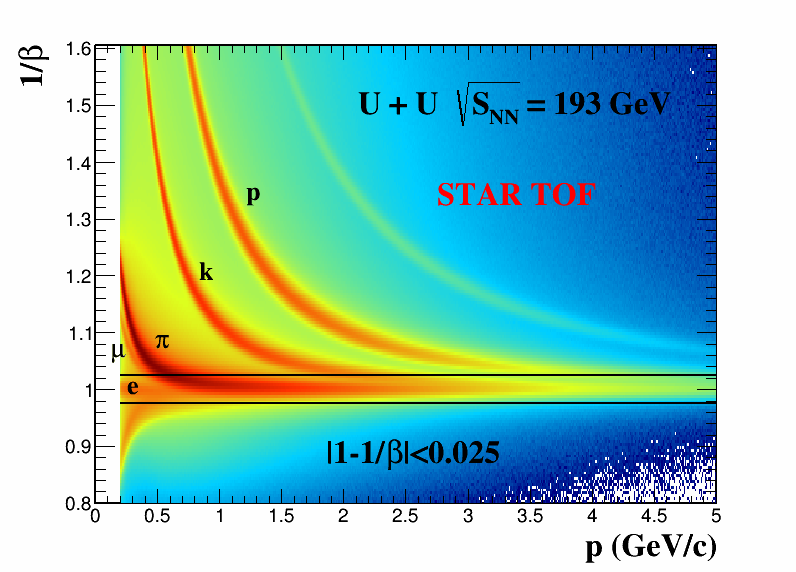
\includegraphics[width=1.0\textwidth]{analysis/betavsp.png}
\caption{$1/\beta$ vs. particle momentum distribution.\label{beta}}
\end{minipage}
\hfill
\begin{minipage}[htbp]{0.48\linewidth}
\centering
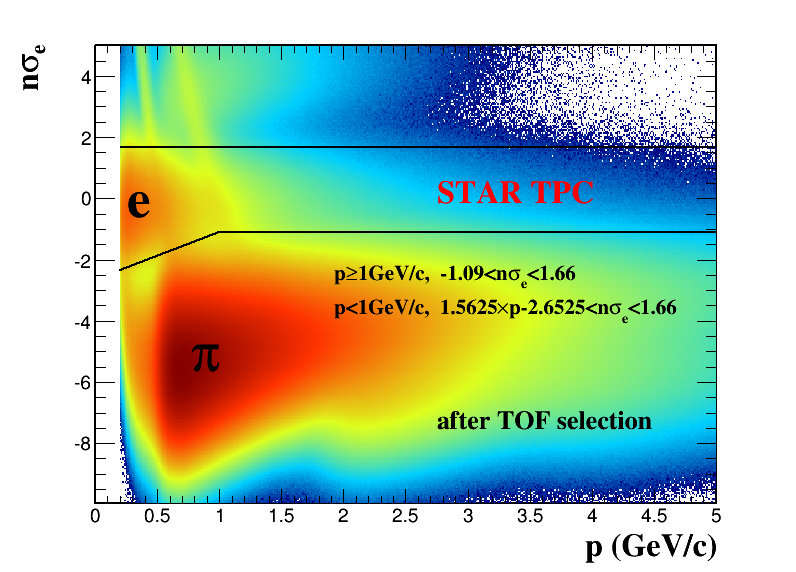
\includegraphics[width=1.0\textwidth]{analysis/nsigmaevsp.png} 
\caption{$n\sigma_{e}$ vs. particle momentum after the high velocity cut applied, as shown in Fig.~\ref{beta}.\label{nsigmae:cut}}
\end{minipage}
\end{figure}

\begin{table}[htp]
\centering
\caption{Electron candidates selection criteria.}
\label{eid}
\newcolumntype{V}{!{\vrule width 1.6pt}}
\begin{tabular}{cVc}
\Xhline{1.6pt}
\thead{\small{Track Quality} \\ \small{Cuts} } &  \thead{ \small{Electron Identification} \\ \small{Cuts} } \\
\Xhline{1.2pt}
0.2 $\leq$ $p_{T}$$\leq$ 30 GeV/$c$ & \multirowcell{2}{p $<$ 1 GeV/$c$, \\ 1.5625$\times$(p - 0.2) - 2 \textbf{- 0.34} $\leq$ $|n\sigma_{e}|$ $\leq$ 2 \textbf{- 0.34}}\\ 
$|\eta|$ $\leq$ 1 & \\ 
nHitsFit $\geq$ 20 & \multirowcell{2}{p $\geq$ 1 GeV/$c$, \\ -0.75 \textbf{- 0.34} $\leq$ $|n\sigma_{e}|$ $\leq$ 2 \textbf{- 0.34}} \\
nHitsFit/nHitsPoss $\geq$ 0.52 & \\ 
nHitsDedx $\geq$ 15 & \multirow{2}*{ $|1 - 1/\beta|$ $\leq$ 0.025} \\
dca $\leq$ 1 cm & \\
\Xhline{1.6pt}
\end{tabular}
\end{table}

\subsection{Electron Purity}
\label{purity}
The pure hadron samples ($\pi/K/p$) are selected by combining tight $m^{2}$ and loose $n\sigma_{hadron}$ cuts. The selection criteria and $n\sigma_{e}$ distribution for each pure hadron sample are shown in Fig.~\ref{purehadron}. The pure electron sample is from the $\pi^{0}$ Dalitz decay and photon conversion. The invariant mass of the electron pair from photon conversion should be zero. However, the primary track, forced to originate from primary vertex, is used to reconstruct the electron pair invariant mass (see detailed procedure in Sec.~\ref{invmass}). That will introduce a artificial opening angle between electron and positron resulting in a non-zero invariant mass. The angle depends on the distance between the photon conversion point and the primary vertex. Thus the photons converting at different positions result in different invariant mass. The $M_{ee} <$ 0.015 GeV/$c^{2}$ is used to select the $\pi^{0}$ Dalitz decayed and photon conversion electrons with 148:1 signal-to-background ratio, shown in the left panel of Fig.~\ref{pheselection}. After subtracting the same sign electron pairs from the opposite sign electron pairs, shown in the right panel of Fig.~\ref{pheselection}, the pure electron sample is thus extracted, shown in Fig.~\ref{pureelectron}. Due to the high charged particle density in U + U collisions at 193 GeV, it is likely to happen that two tracks with same charge and similar momentum are very closed to each other. The two tracks are very likely to be reconstructed into ``one track'' due to the finite hit position resolution, so called ``merged track''. The pion is very abundant in U + U collisions at 193 GeV, thus the ``merged $\pi$'' should be taken into account for the purity study. The ``merged $\pi$'' could be selected using the same $m^{2}$ cut as normal $\pi$ but with $n\sigma_{\pi} >$ 6 (``merged $\pi$'' is with doubled $dE/dx$ compared to a normal $\pi$). The $n\sigma_{e}$ distribution of each selected pure sample could be fitted by Gaussian function in each fine $p_{T}$ bin. The mean and sigma of the $n\sigma_{e}$ distribution for each pure sample are shown in Fig.~\ref{puresamplemeansigma}. The electron purity is then estimated based on multi-Gaussian fitting while the mean and width of each component is constrained by the values in Fig.~\ref{puresamplemeansigma}. Figure~\ref{multigaus} shows an example of the multi-Gaussian fitting. In the $dE/dx$ overlap region, the multi-Gaussian fitting is not reliable. An exponential function is employed to extrapolate the hadron particle yields in the overlapping regions as shown in the left panel of  Fig.~\ref{particleyield}. The hadron yields are then constrained, just leaving the electron yield as a free parameter, in the multi-Gaussian function for refitting. The electron yield from the second-round multi-Gaussian fitting is extracted to check the fit reliability, shown in the right panel of Fig.~\ref{particleyield}. The electron purity difference between these two-round fittings is taken as the systematic uncertainty. Figure~\ref{electronpurity} shows the electron purity (overall at $\sim$95\%) in U + U minimum-bias collisions at 193 GeV.

\begin{figure}
\centering
\vspace*{-3mm}
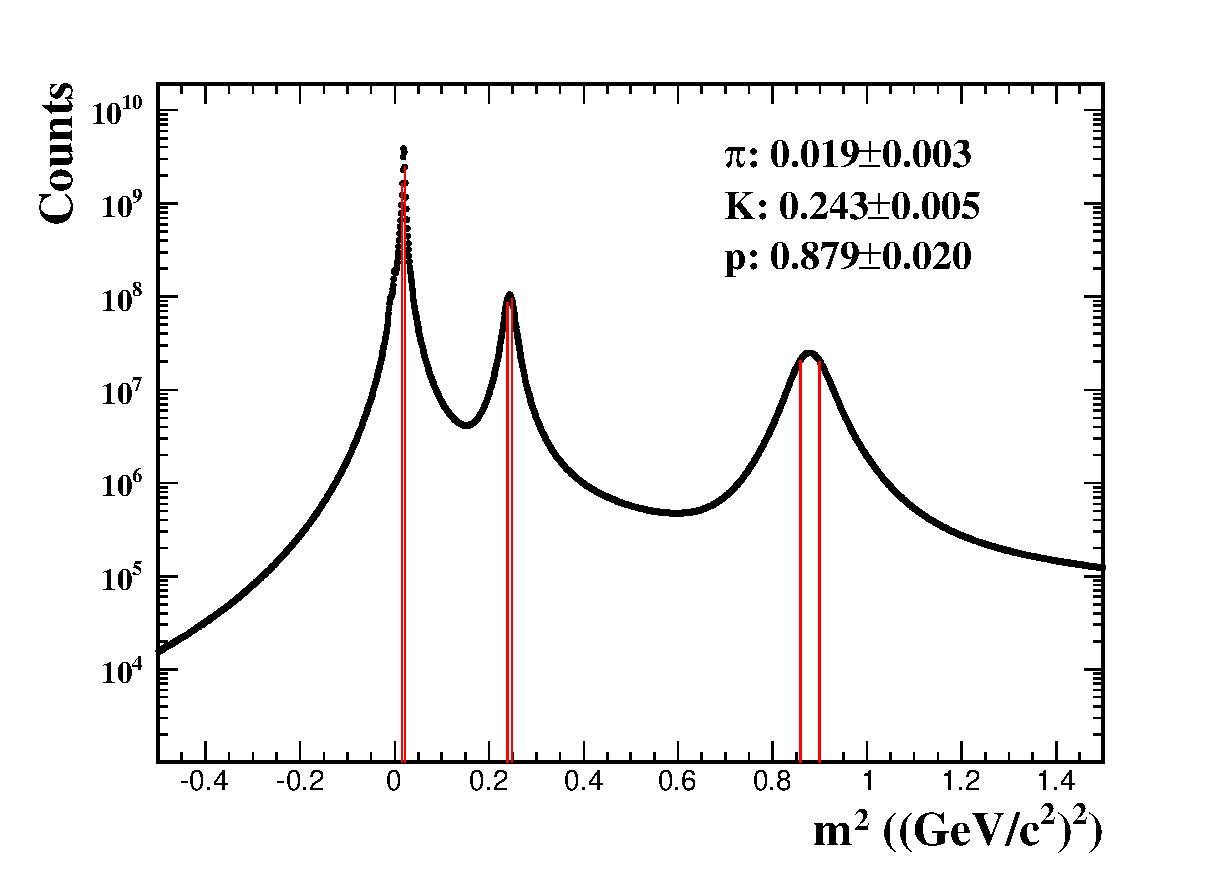
\includegraphics[width=0.48\textwidth]{analysis/pikpsample.eps}
\hspace*{-5mm}
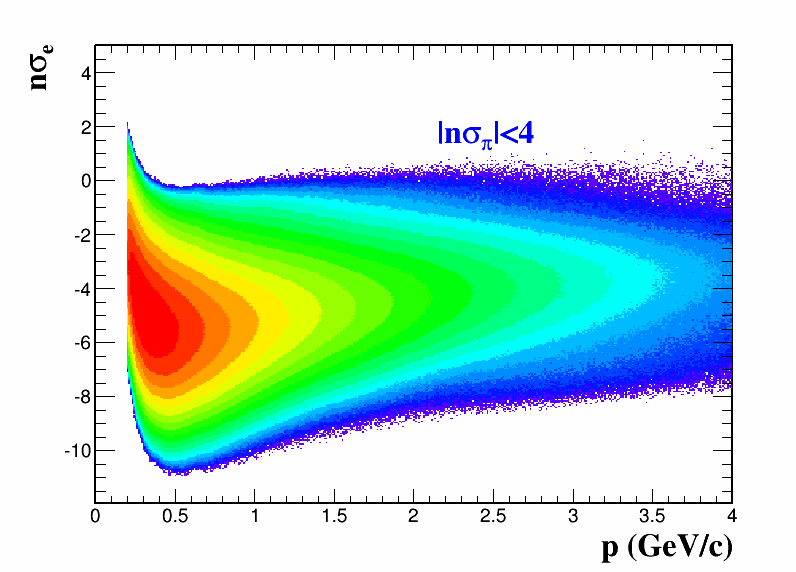
\includegraphics[width=0.48\textwidth]{analysis/PinSigEvsP.png}
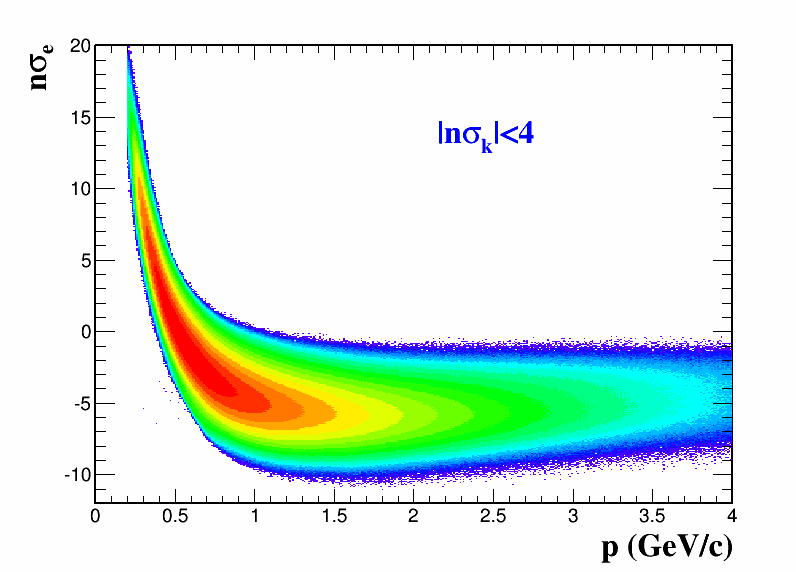
\includegraphics[width=0.48\textwidth]{analysis/knSigEvsP.png}
\hspace*{-5mm}
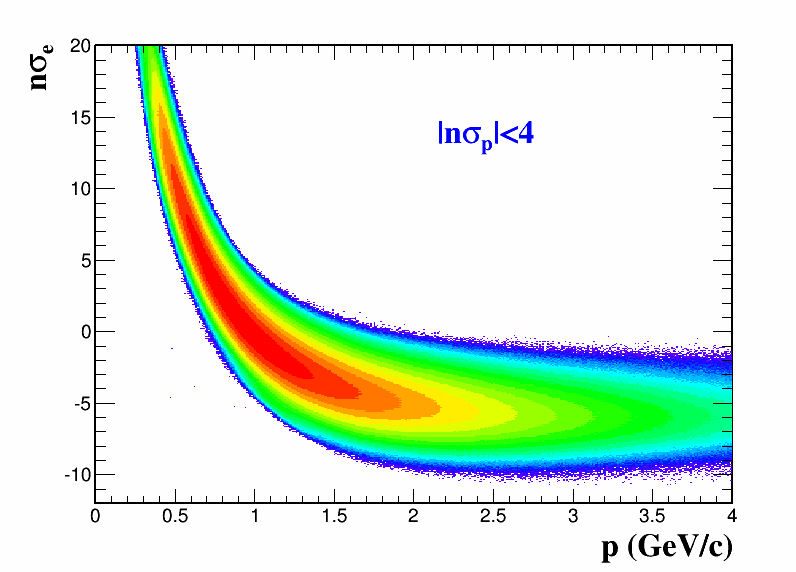
\includegraphics[width=0.48\textwidth]{analysis/PnSigEvsP.png}
\figcaption{The selection criteria and $n\sigma_{e}$ distribution as a function of momentum for each pure hadron sample in U + U 193 GeV minimum-bias collisions. (Top Left) $m^{2}$ distribution of different particle species and pure hadron $m^{2}$ selection criteria. (Top Right) Pure pion sample. (Bottom Left) Pure kaon sample. (Bottom Right) Pure proton sample.}
\label{purehadron}
\end{figure}

\begin{figure}
\centering
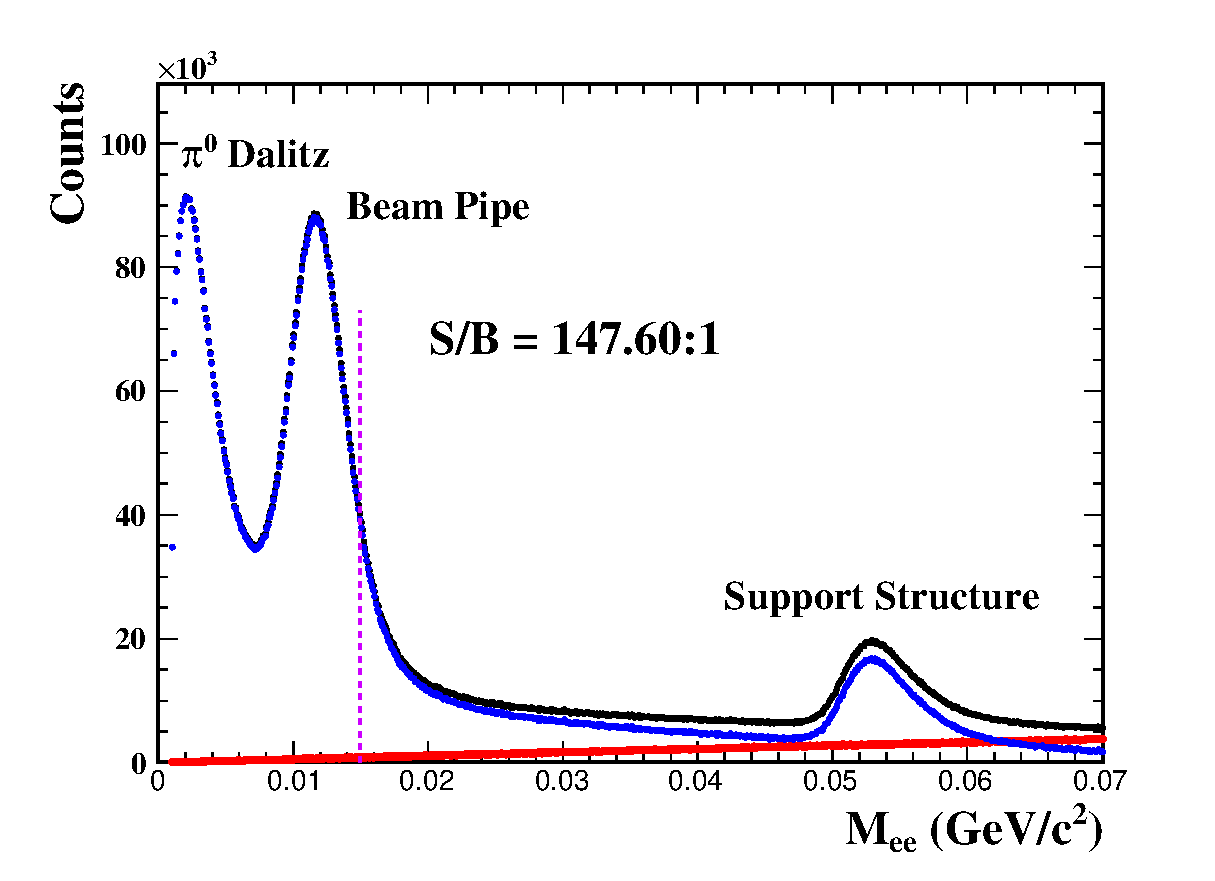
\includegraphics[width=0.48\textwidth]{analysis/PHE.eps}
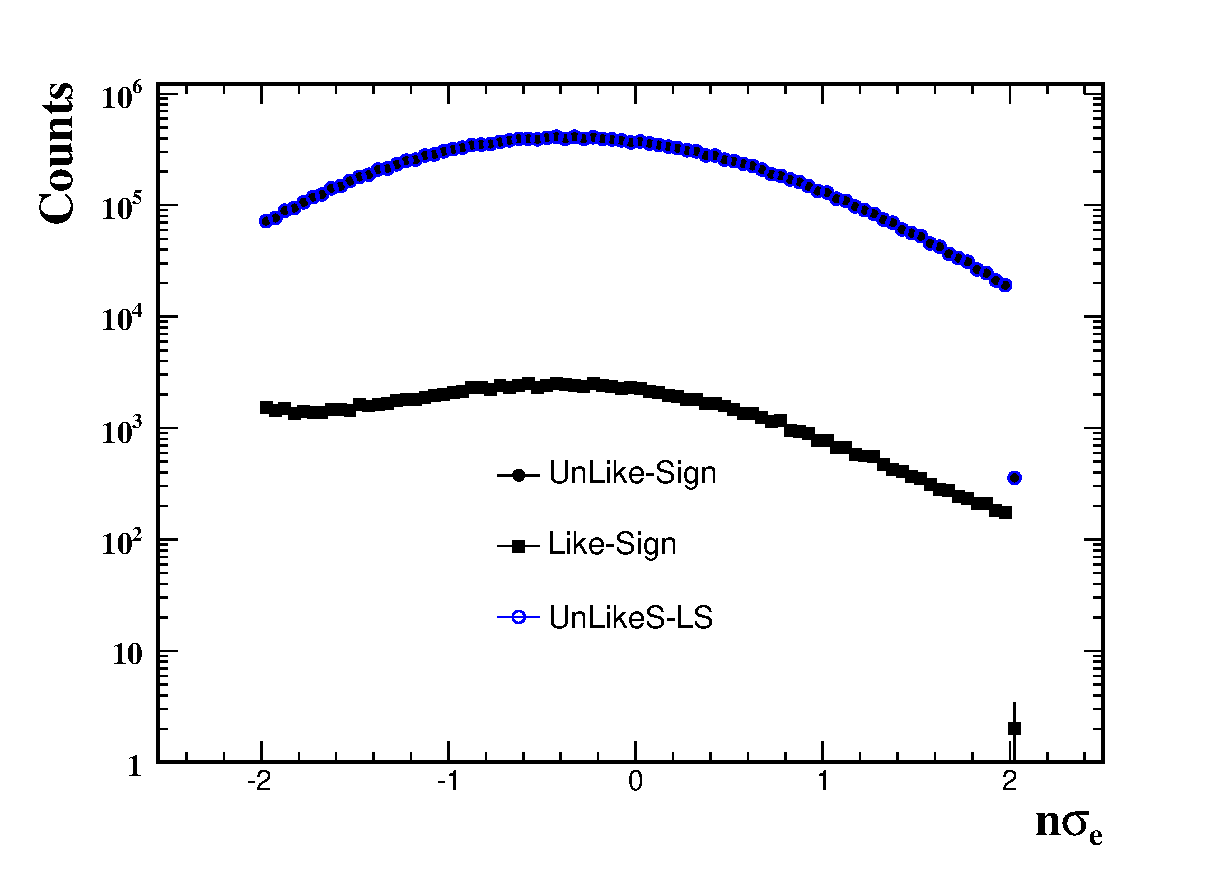
\includegraphics[width=0.48\textwidth]{analysis/PHE_UL_Like.eps}
\figcaption{The selection criteria and $n\sigma_{e}$ distribution of pure electron sample in U + U minimum-bias collisions at 193 GeV. (Left) The invariant mass distribution of $\pi^{0}$ Dalitz decay and photon conversion electron pairs. (Right) The $n\sigma_{e}$ distribution of $\pi^{0}$ Dalitz decay and photon conversion electrons.}
\label{pheselection}
\end{figure}

\begin{figure}[htbp]
\centering
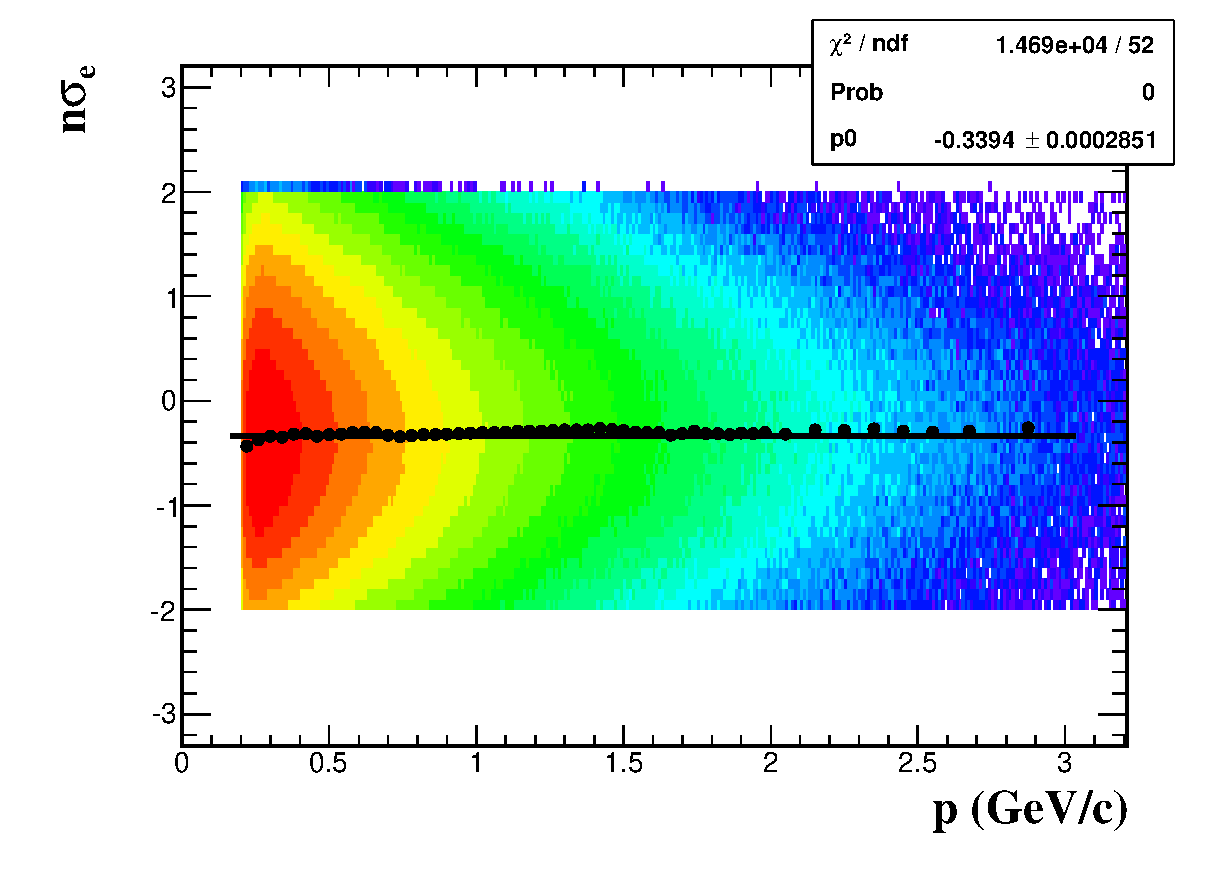
\includegraphics[keepaspectratio,width=0.6\textwidth]{analysis/mean_of_nsigmae_vs_pt_4electron.eps}
\figcaption{The $n\sigma_{e}$ distribution of pure electron sample as a function of momentum in U + U minimum-bias collisions at 193 GeV. The mean of the $n\sigma_{e}$, shown as black dots, is shift to -0.34 due to imperfect TPC $dE/dx$ calibration.}
 \label{pureelectron}
\end{figure}

\begin{figure}
\centering
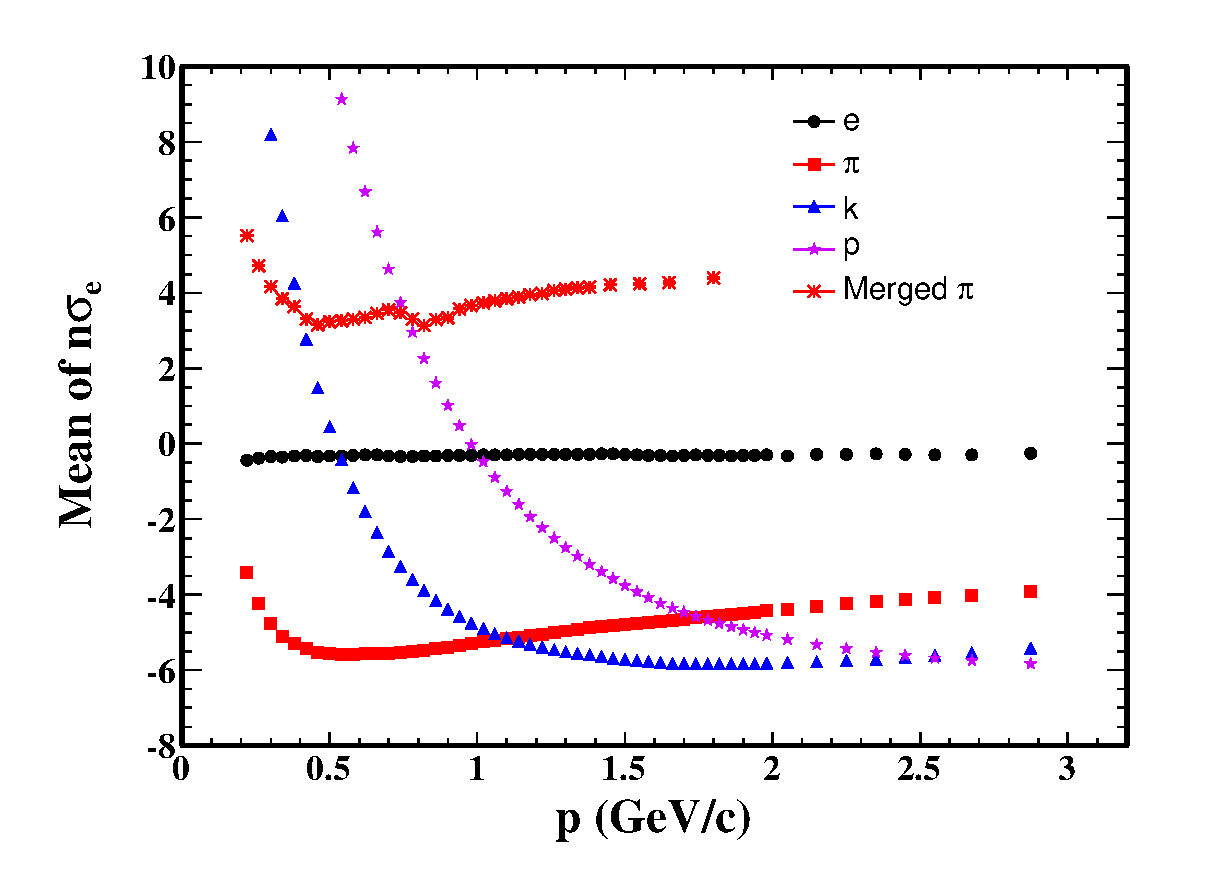
\includegraphics[width=0.48\textwidth]{analysis/mean_of_nsigmae_vs_pt.eps}
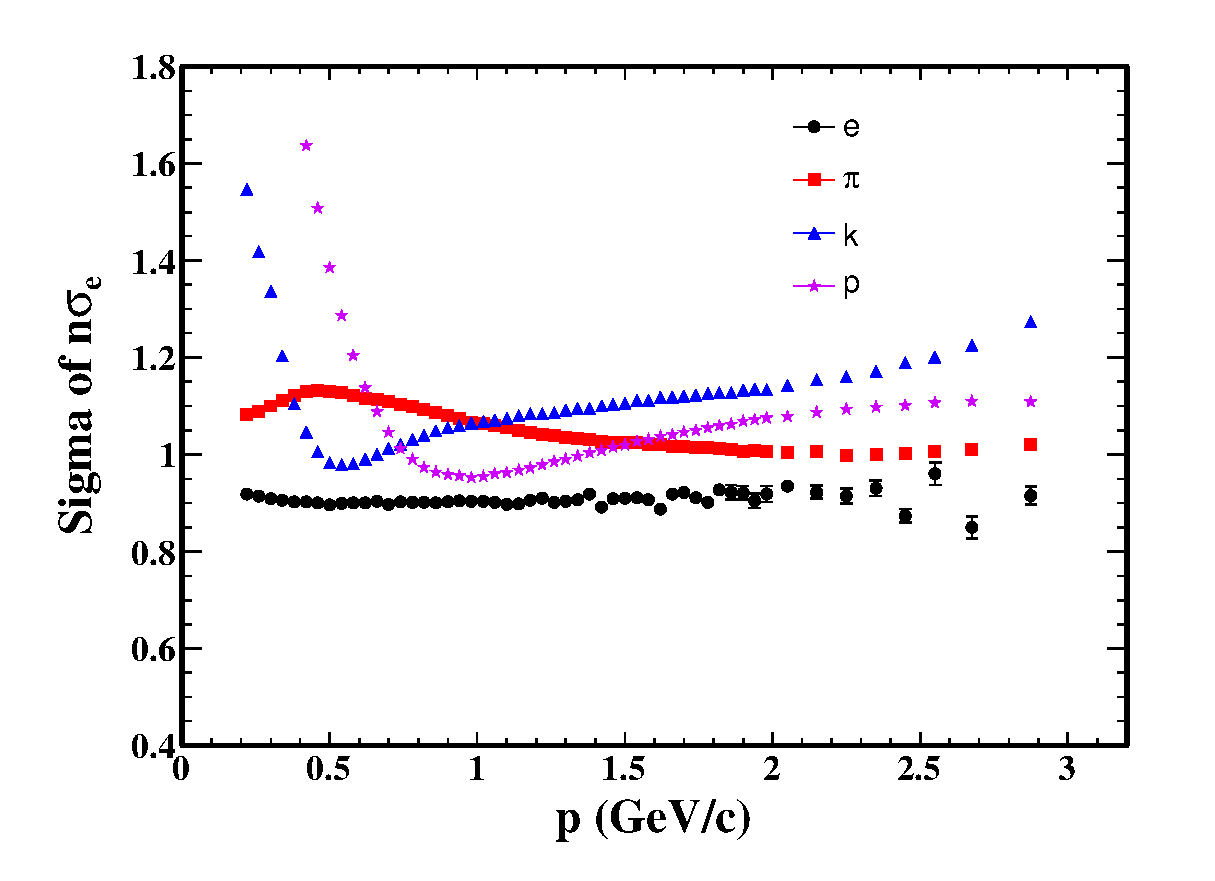
\includegraphics[width=0.48\textwidth]{analysis/sigma_of_nsigmae_vs_pt.eps}
\figcaption{The mean (Left) and sigma (Right) of the $n\sigma_{e}$ for each pure particle sample as a function of momentum in U + U 193 GeV minimum-bias collisions.}
\label{puresamplemeansigma}
\end{figure}

\begin{figure}[htbp]
\centering
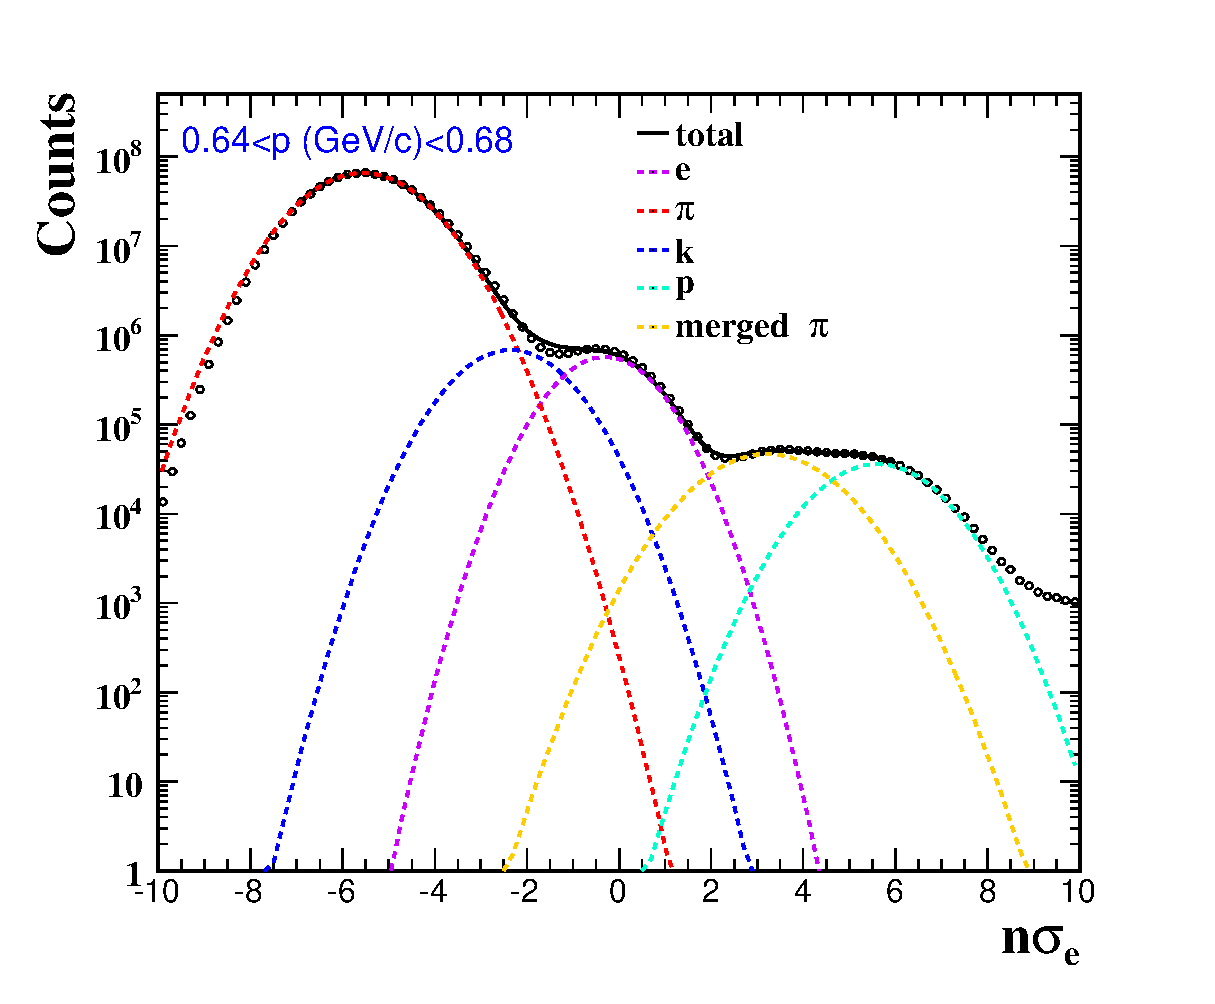
\includegraphics[keepaspectratio,width=0.5\textwidth]{analysis/multi_Gaussian_fit.eps}
\figcaption{The $n\sigma_{e}$ distribution after the TOF velocity cut and the multi-Gaussian fit result in momentum bin (0.64, 0.68) GeV/$c$.}
 \label{multigaus}
\end{figure}

\begin{figure}[htbp]
\centering
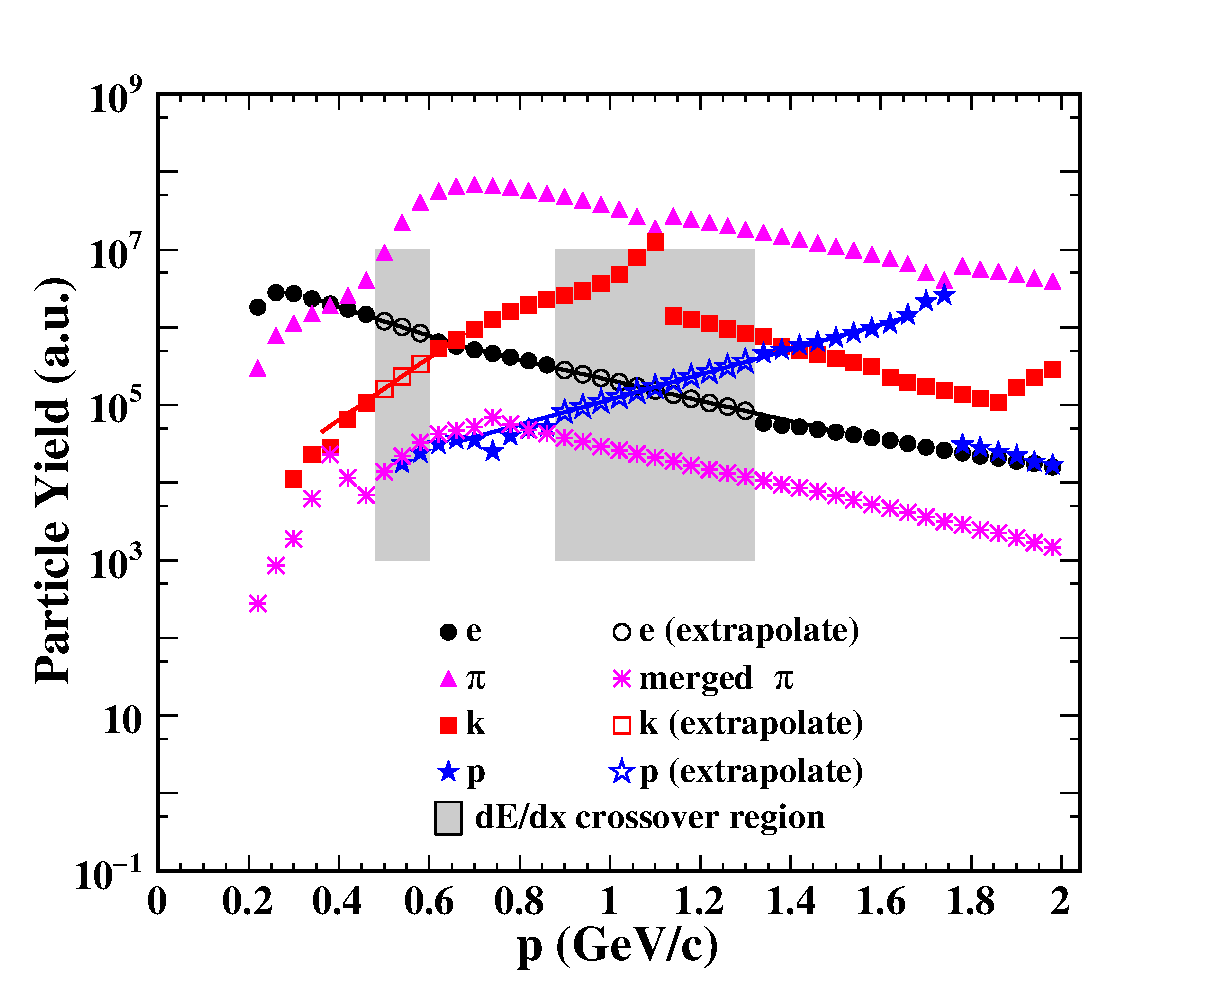
\includegraphics[width=0.48\textwidth]{analysis/Fit_Interpolate_ConstValue.eps}
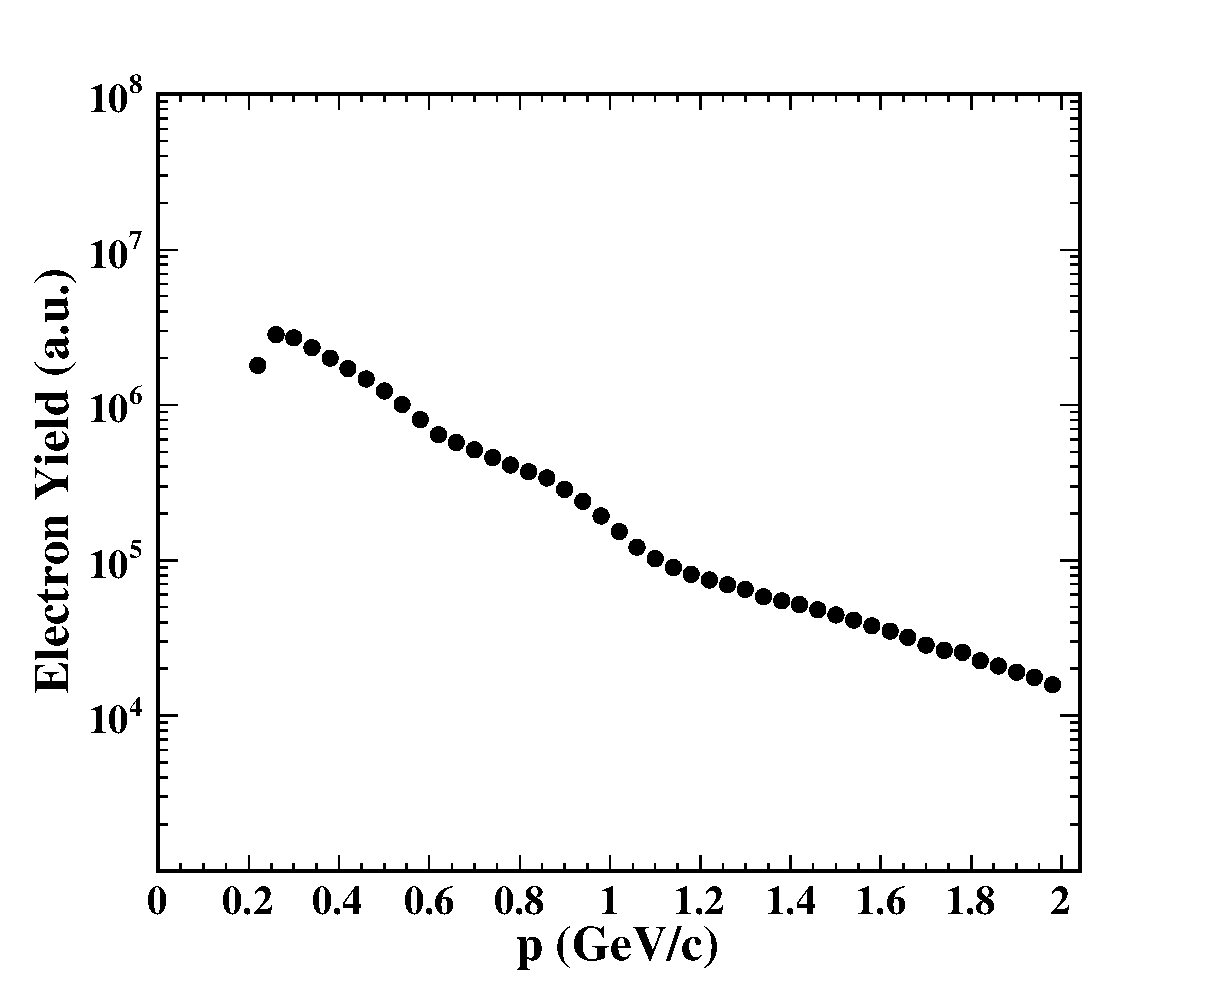
\includegraphics[width=0.48\textwidth]{analysis/Econst_crosscheck.eps}
\figcaption{(Left) The yields (solid markers) for different particle species extracted from first-round multi-Gaussian fitting as a function of momentum. The gray areas (left: $e/K$, right: $e/p$) depict the $dE/dx$ crossover regions. The solid lines are the exponential fits for extrapolating the hadron yields (open markers) in the crossover regions. (Right) The electron yields (the only free parameter) from the second-round multi-Gaussian fitting to check the fitting reliability.}
\label{particleyield}
\end{figure}

\begin{figure}[htbp]
\centering
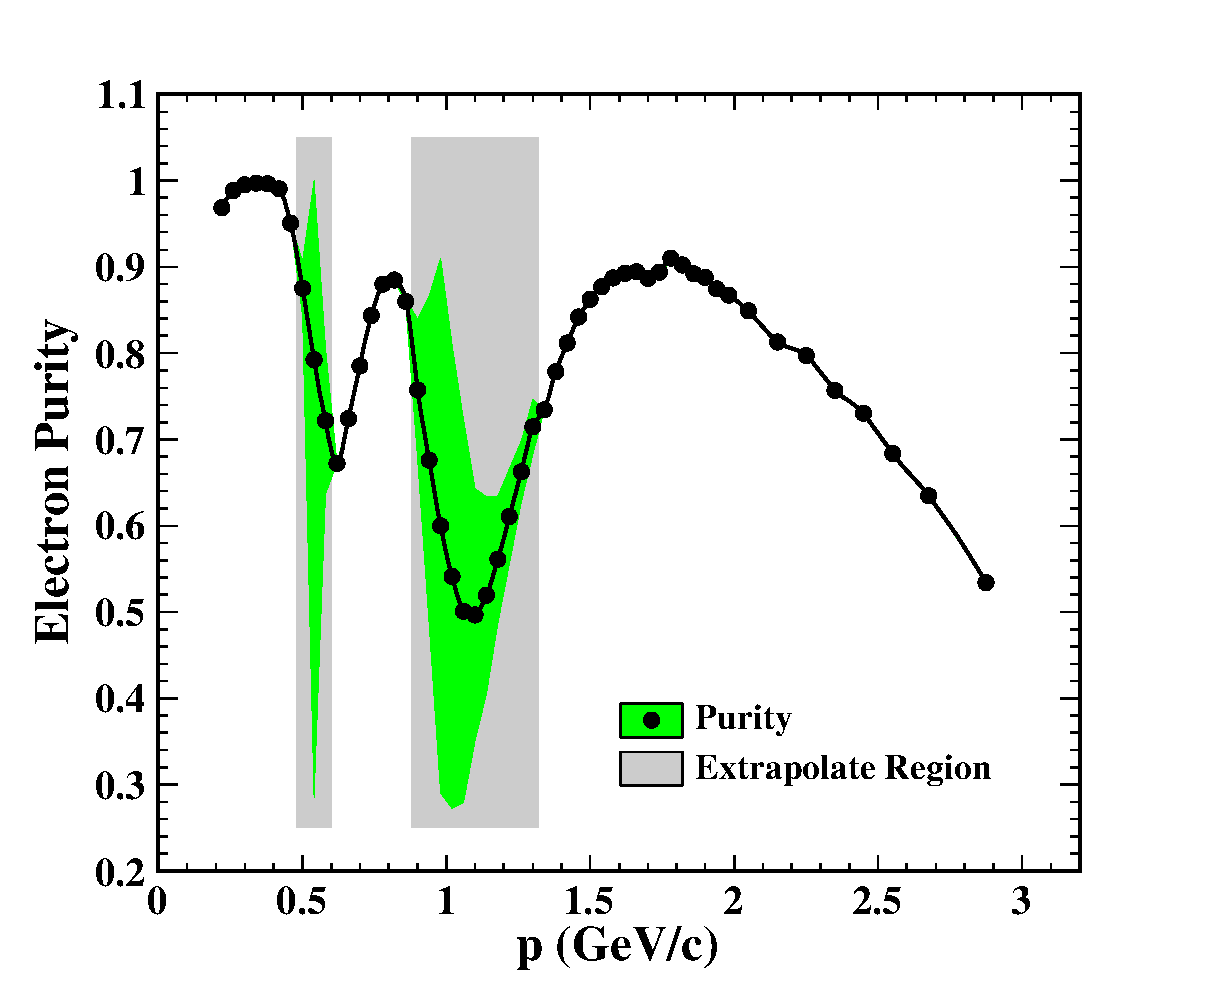
\includegraphics[keepaspectratio,width=0.5\textwidth]{analysis/Electron_Pur.eps}
\figcaption{The electron purity in U + U minimum-bias collisions at 193 GeV, the green band represents the systematic uncertainties.}
 \label{electronpurity}
\end{figure}


\section{Pair Reconstruction and Background Subtraction}
\label{invmass}
The foreground (also called unlike-sign pairs, $N_{+-}$, including signal and background) is reconstructed by combining the electron and positron candidates in the same event. The invariant mass ($M_{ee}$) of the electron pairs are calculated by Eq.~\ref{mass}, 
\begin{equation}
M_{ee} = \sqrt{ (E_{+} + E_{-})^{2} - (\overrightarrow{p}_{+} + \overrightarrow{p}_{-})^{2}}
\label{mass}
\end{equation}
where $E_{+/-} = \sqrt{m_{e}^{2} + \overrightarrow{p}_{+/-}^{2}}$, $m_{e}$ = 0.511 MeV/$c^{2}$ and $\overrightarrow{p}_{+/-}$ are measured by the TPC. The signals come from the Drell-Yan production, quarkonia decay, QGP thermal radiation, heavy flavor semi-leptonic decay, vector mesons in-medium decay and long-lived hadron decays. The background sources include the combinatorial background, correlated background and photon conversions. The combinatorial background comes from uncorrelated electron and positron pairing while the correlated background comes from correlated electron and positron pairing; for example, pairs from Dalitz decay followed by a conversion of the decayed photon (e.g. $\pi^{0} \rightarrow \gamma + e^{+} + e^{-} \rightarrow e^{+} + e^{-} + e^{+} + e^{-}$) or jets (e.g. electron and positron are from same-jet fragmentation or back-to-back di-jet fragmentation). The photon conversion background is from the photon interacting with the detector material and converting into an electron-positron pair. The reconstruction and subtraction of these three background sources are discussed in following sections.

%\begin{figure}[htbp]
%\centering
%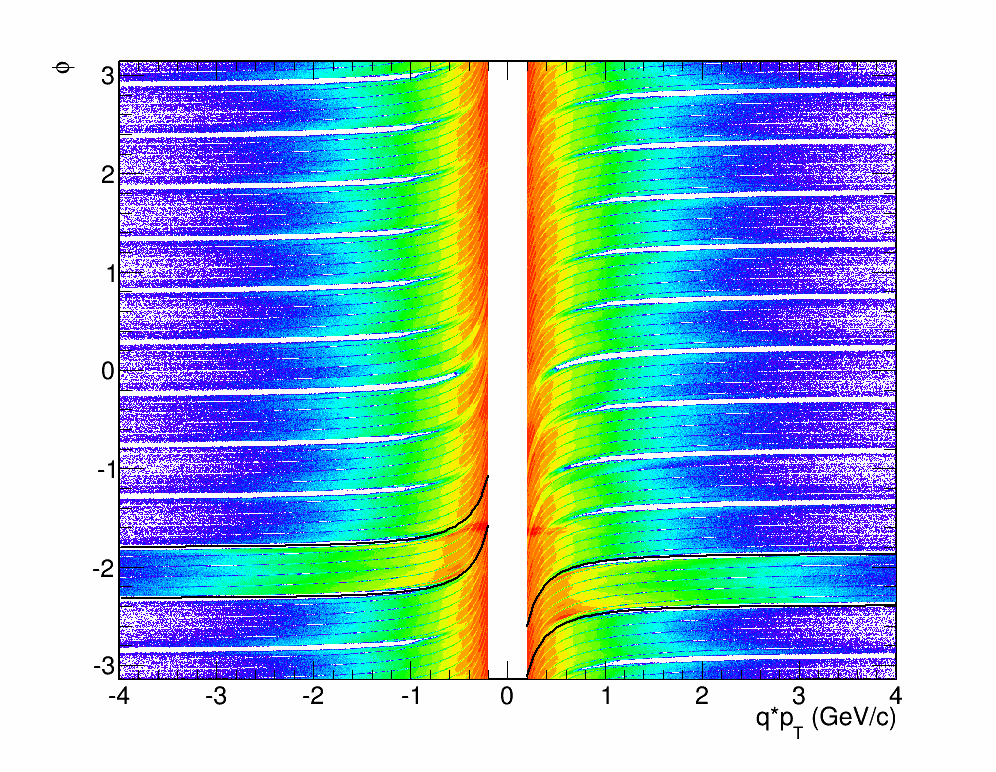
\includegraphics[keepaspectratio,width=1.0\textwidth]{analysis/hephivsp.png}
%\figcaption{The $\phi$ vs. $p_{T}$ distributions for electron and positron candidates. The blank strips are caused by the read-out sector boundaries. The bad TPC sector (sector 7, in positive $\eta$ region) is constrained by the black solid lines.}
% \label{ephivspt}
%\end{figure}

\begin{figure}[htbp]
\begin{minipage}[htbp]{0.49\linewidth}
\centering
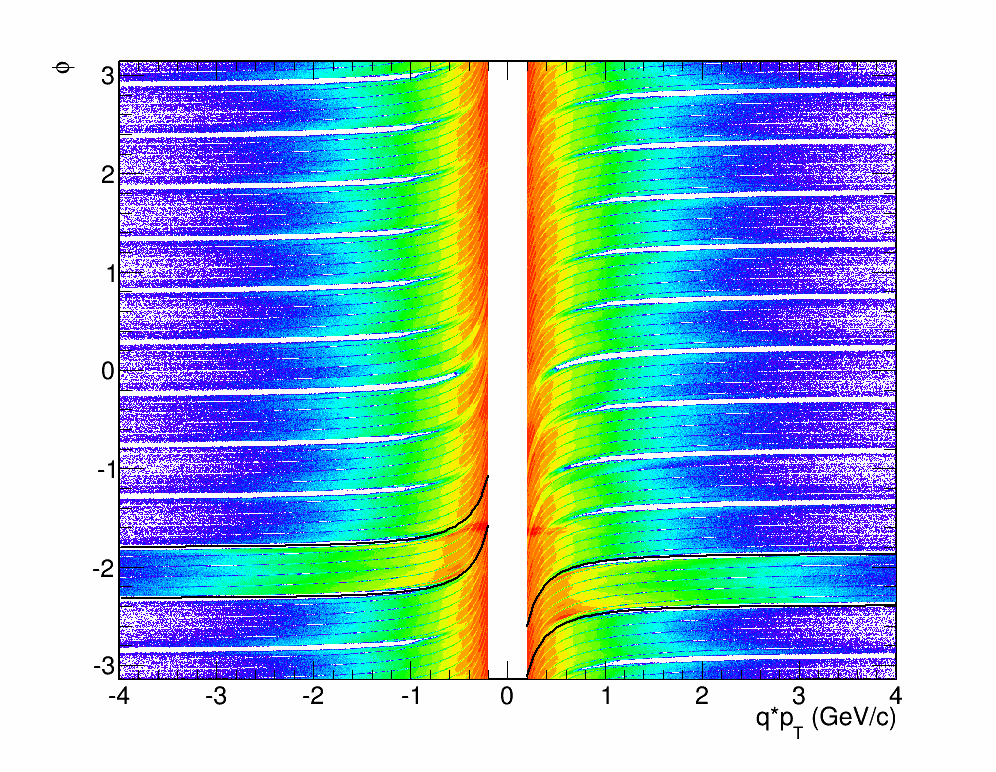
\includegraphics[width=1.0\textwidth]{analysis/hephivsp.png}
\caption{The $\phi$ vs. $p_{T}$ distributions for electron and positron candidates. The blank strips are caused by the read-out sector boundaries. The bad TPC sector (sector 7, in positive $\eta$ region) is constrained by the black solid lines.\label{ephivspt}}
\end{minipage}
\hfill
\begin{minipage}[htbp]{0.49\linewidth}
\centering
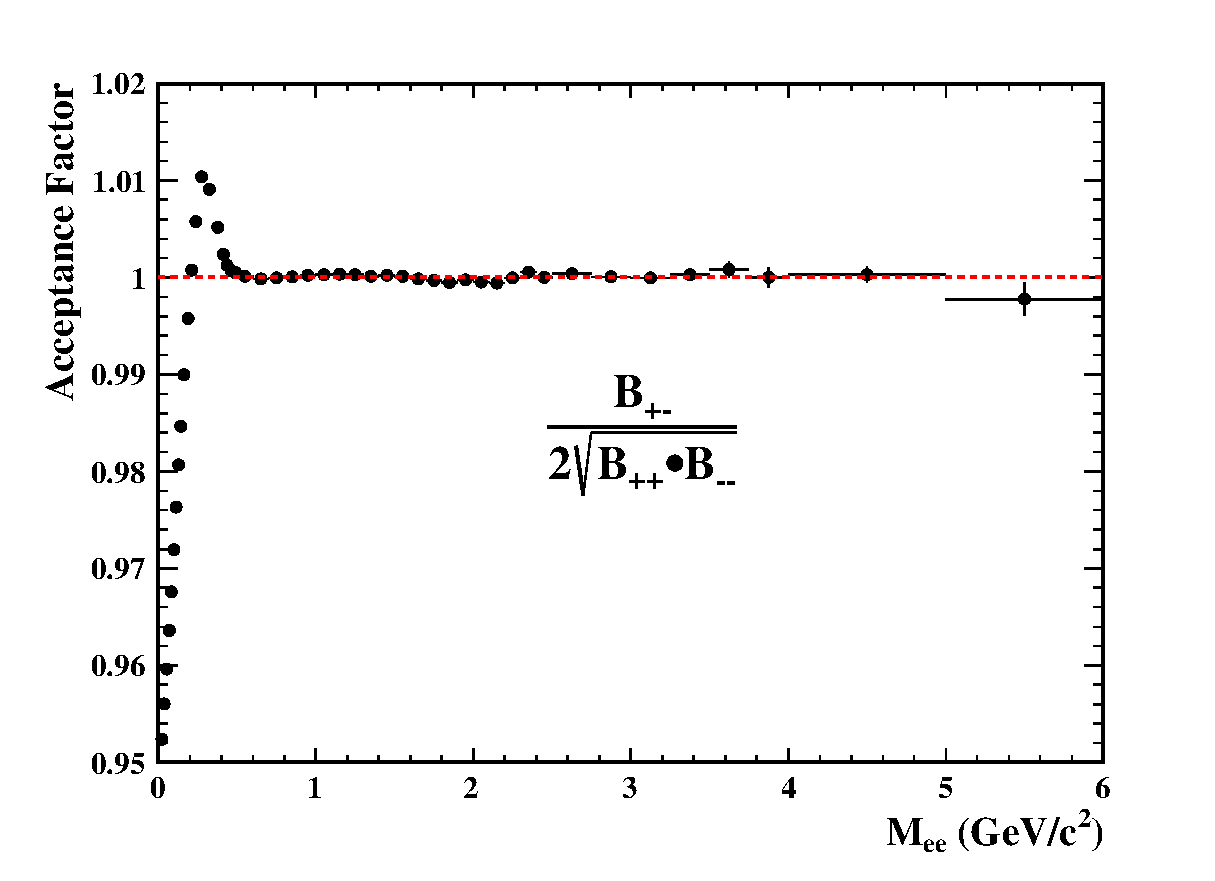
\includegraphics[width=1.0\textwidth]{analysis/acceptance1D.eps} 
\caption{The 1-D acceptance correction factor as a function of $M_{ee}$ in Run12 U + U  minimum-bias collisions at 193 GeV.\label{acc1d}}
\end{minipage}
\end{figure}

\subsection{Like-sign Technique}
\label{likesign}

The like-sign technique, combining same charge sign electrons into pairs in the same event ($N_{++}$ and $N_{--}$), is used to account for the combinatorial and correlated backgrounds. The geometric mean of the like-sign pairs 2$\sqrt{N_{++} \bm\cdot N_{--}}$, demonstrated  in~\cite{PHENIX:dielectron0}, can fully describe the background in the foreground when the $e^{+}$ and $e^{-}$ are produced in statistically independent pairs. The geometric mean is consistently used in the same-event like-sign background reconstruction. 

%\begin{figure}[htbp]
%\centering
%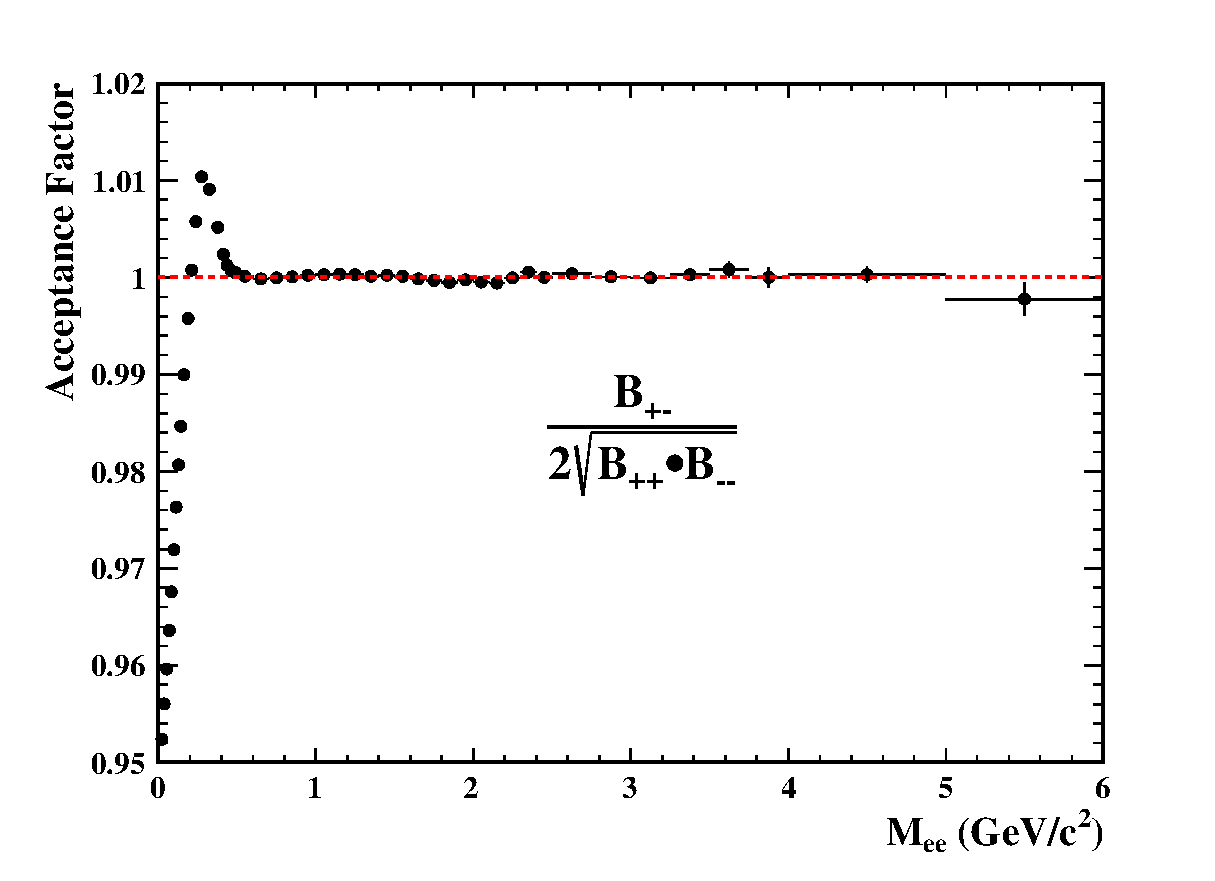
\includegraphics[keepaspectratio,width=0.8\textwidth]{analysis/acceptance1D.eps}
%\figcaption{The 1-D acceptance correction factor as a function of $M_{ee}$ in Run12 U + U  minimum-bias collisions at 193 GeV.}
 %\label{acc1d}
%\end{figure}

The electrons and positrons are bended into opposite directions owing to the magnetic field. The $\phi$ versus $p_{T}$ of the identified electron and positron candidates is shown in Fig.~\ref{ephivspt}. The blank strips along the $\phi$ direction are caused by the TPC read-out sector boundaries. There is one TPC sector (sector 7, in positive $\eta$ region) with $dE/dx$ calibration issue in Run12 U + U collisions, depicted by the black solid lines in Fig.~\ref{ephivspt}. Thus all the tracks passing through this TPC sector are consistently rejected in this analysis. Due to the magnetic field and the TPC de-active areas (read-out sector boundaries, acceptance holes), the acceptances for the unlike-sign and like-sign pairs are different. The mixed-event technique, discussed in Sec.~\ref{mixedevent}, is employed to correct for this effect. The correction factor is calculated by the ratio of the mixed-event unlike-sign and like-sign distribution in each ($M_{ee}$, $p_{T}^{ee}$) bin and applied in 2-dimension (2-D). The final same-event like-sign background used is calculated by the Eq.~\ref{corrlikesign}, 
\begin{equation}
N_{++\&--}^{corr} = 2\sqrt{N_{++}(M, p_{T}) \bm\cdot N_{--}(M,p_{T})} \times \frac{B_{+-}(M,p_{T})}{2\sqrt{B_{++}(M, p_{T}) \bm\cdot B_{--}(M,p_{T})}}
\label{corrlikesign}
\end{equation}
where $N_{++}$, $N_{--}$, $B_{++}$, and $B_{--}$ represent the distribution of like-sign from the same-event and mixed-event, respectively. $B_{+-}$ represents the distribution of unlike-sign from the mixed-event. $N_{++\&--}^{corr}$ denotes the acceptance-corrected like-sign background from the same-event. Figure~\ref{acc1d} shows the 1-D acceptance correction factor as a function of $M_{ee}$ in Run12 U + U minimum-bias collisions at 193 GeV. 

\subsection{Mixed-Event Technique}
\label{mixedevent}
The like-sign technique, discussed in Sec.~\ref{likesign}, is taken as the best estimation for the combinatorial and correlated backgrounds. However, it is limited to the statistics. The mixed-event technique, combining the electrons and positrons from different events with similar characteristics, is used to reproduce the combinatorial background with improved statistical precision. The data sample is divided into different event pools according to the following event level properties: $z$ position of collision vertex, reference multiplicity, and event plane angle. The collision vertex position and reference multiplicity ensure that the same event pool has similar detector acceptance and efficiency. The event plane angle ensures the same event pool has similar momentum phase space alignment, and further guaranteed by the multiplicity assortment to ensure the events have similar momentum phase space distribution. The second-order event plane angle~\cite{EventPlane0, EventPlane1} is used to sort the events. The $z$ vertex position, form -30 cm to +30 cm, is divided into 10 equidistant bins. The reference multiplicity is divided into 16 bins (0 - 80\%, discussed in Sec.~\ref{centrality}) according to the official StRefMult package provided by STAR. The event plane angle $\Psi$ is divided into 24 equidistant bins. This granularity of the event pools is determined by the same procedure discussed in~\cite{STAR:dielectron1,dielectronJie}. Each event pool holds 100 events at maximum, and one event in the event pool is randomly updated when the pool is full. 

The mixed-event background must be normalized to the acceptance corrected same-event like-sign background. The mixed-event technique can not reproduce the correlated background, thus the normalization factor should be determined in a kinematic region where the same-event like-sign correlated background is negligible. Once the kinematic region selected, the normalization factor and the normalized combinatorial background ($B_{+-}^{comb}$) are calculated via the same method in~\cite{PHENIX:dielectron0} and also shown in Eq.~\ref{normalization}
\begin{equation}
\begin{split}
A_{+} = \frac{\int_{N.R.}N_{++}(M,p_{T})dMdp_{T}}{\int_{N.R.}B_{++}(M,p_{T})dMdp_{T}} \\
A_{-} = \frac{\int_{N.R.}N_{--}(M,p_{T})dMdp_{T}}{\int_{N.R.}B_{--}(M,p_{T})dMdp_{T}} \\
B_{++}^{norm} = \int_{0}^{\infty}A_{+}B_{++}(M,p_{T})dMdp_{T} \\
B_{--}^{norm} = \int_{0}^{\infty}A_{-}B_{--}(M,p_{T})dMdp_{T} \\
B_{+-}^{comb}(M,p_{T}) = \frac{2\sqrt{B_{++}^{norm}B_{--}^{norm}}}{\int_{0}^{\infty}B_{+-}(M,p_{T})dMdp_{T}}B_{+-}(M,p_{T}) 
\label{normalization}
\end{split}
\end{equation}
where N.R. represents the normalization region, $A_{+/-}$ is the like-sign normalization factor in N.R., $B_{++/--}^{norm}$ is the normalized mixed-event like-sign statistics and $B_{+-}^{comb}$ is the normalized mixed-event unlike-sign distribution. Unfortunately the mixed-event technique, working in Au + Au at 200 GeV, does not work in U + U at 193 GeV. There is no flat kinematic region found to do the normalization, as shown in Fig.~\ref{likemixratio}. This may be related to the asymmetric Uranium geometry compared to the symmetric Gold geometry, shown in Fig.~\ref{geometry}. Thus, the same-event like-sign technique is finally used to reconstruct the background in this analysis.

\begin{figure}[htbp]
\centering
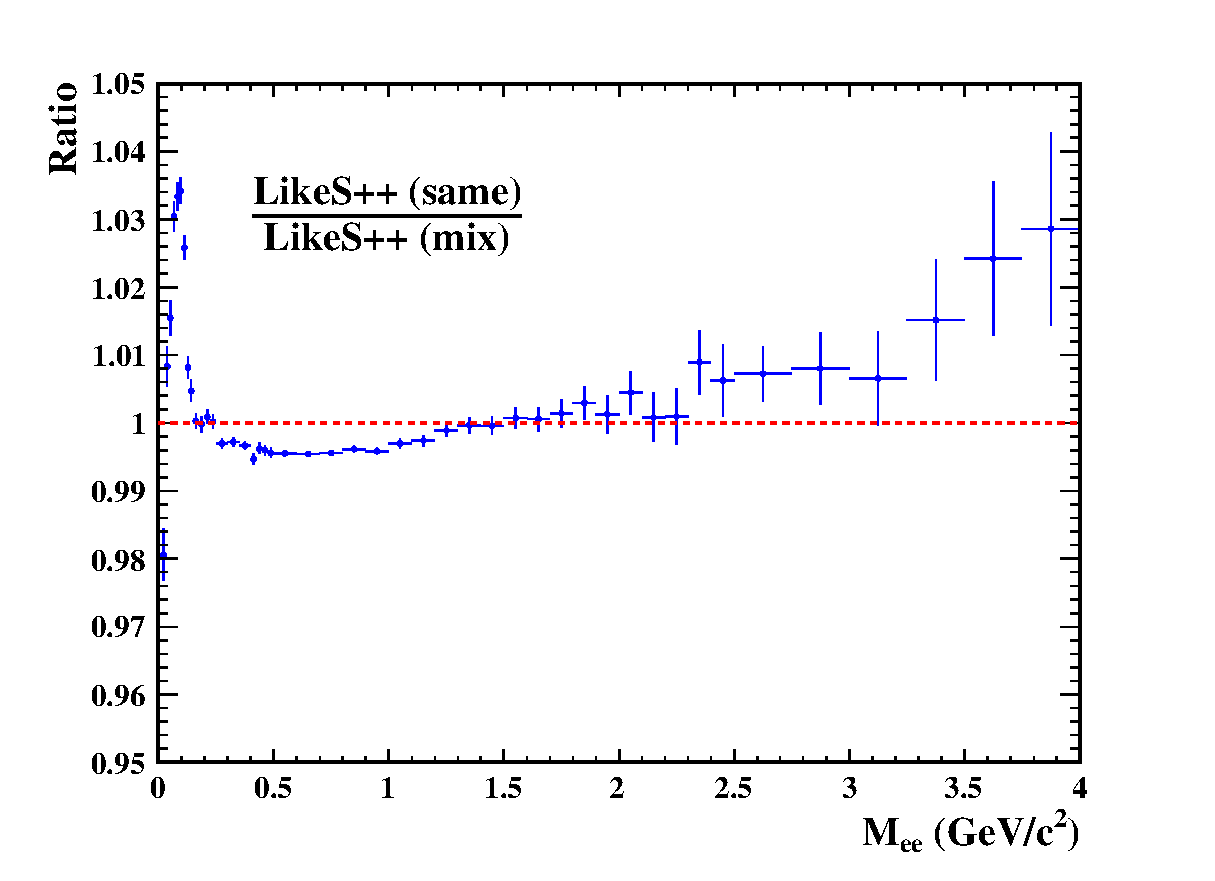
\includegraphics[width=0.48\textwidth]{analysis/LMixPosRatio1D.eps}
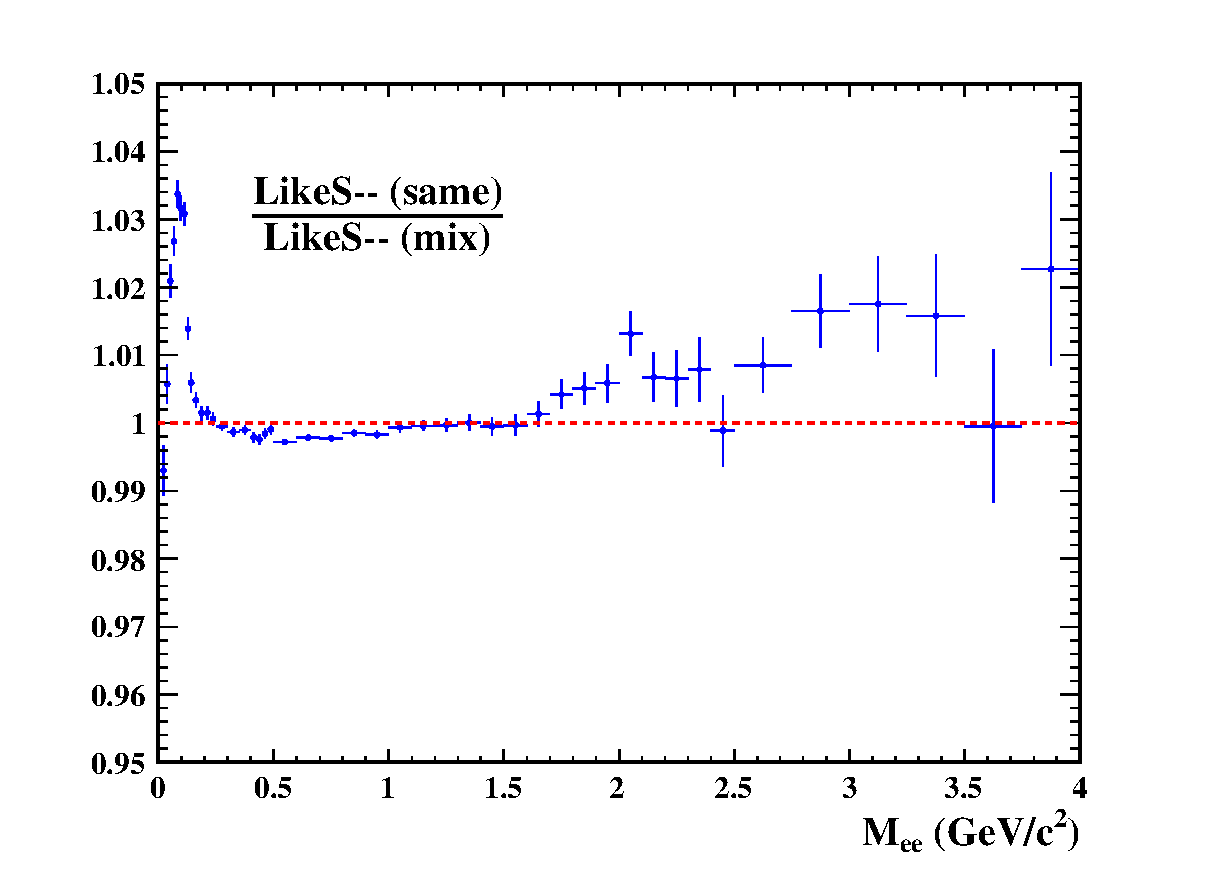
\includegraphics[width=0.48\textwidth]{analysis/LMixNegRatio1D.eps}
\figcaption{Ratios between same-event and mixed-event like-sign distributions. There is no flat kinematic region to do the mixed-event normalization.}
\label{likemixratio}
\end{figure}

\begin{figure}[htbp]
\centering
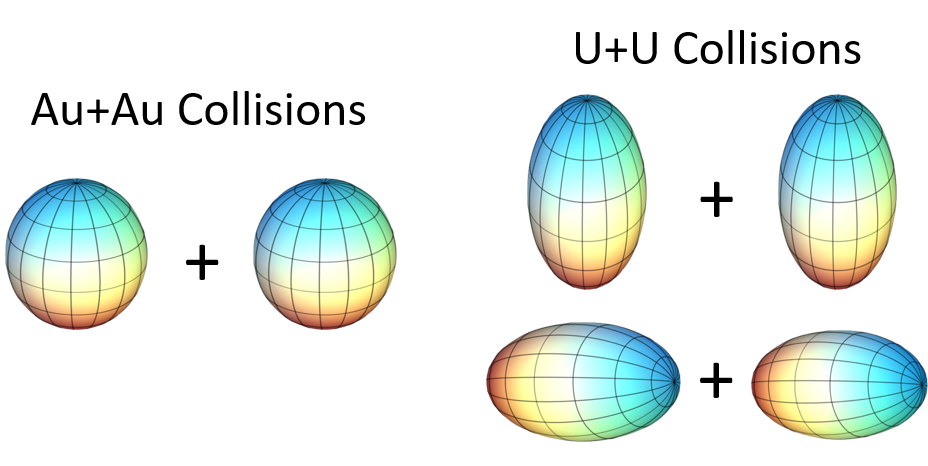
\includegraphics[keepaspectratio,width=0.7\textwidth]{analysis/UUGeometry.png}
\figcaption{The spherical Gold nuclei (Left) and the ellipsoidal Uranium nuclei (Right).}
 \label{geometry}
\end{figure}

\subsection{Photon Conversion Removal}
The photon conversion electron pairs are removed from the foreground using the $\phi_{V}$ cut method which is similar to that used by the PHENIX Collaboration~\cite{PHENIX:dielectron0}. The opening angle between the electron and positron from the photon conversion should be 0, and the electron and positron are bent only in the plane perpendicular the magnetic field direction which is along the beam axis $z$ in STAR. The definitions of the unit vector and $\phi_{V}$ angle are shown in the following Eq.~\ref{phiv:eq}:
\begin{equation}
\begin{split}
\stackrel{\wedge}{u}\;= \frac{\overrightarrow{p}_{+} + \overrightarrow{p}_{-}}{|\overrightarrow{p}_{+} + \overrightarrow{p}_{-}|}, \quad
\stackrel{\wedge}v\;= \overrightarrow{p}_{+} \times \overrightarrow{p}_{-} \\
\stackrel{\wedge}w\;=\;\stackrel{\wedge}u \times \stackrel{\wedge}v, \quad
\stackrel{\wedge}w_{c}\;=\;\stackrel{\wedge}u \times \stackrel{\wedge}z \\
cos\phi_{V} = \frac{\stackrel{\wedge}w}{|\stackrel{\wedge}w|} \cdot \frac{\stackrel{\wedge}w_{c}}{|\stackrel{\wedge}w_{c}|}
\label{phiv:eq}
\end{split}
\end{equation}

\begin{figure}[htbp]
\begin{minipage}[htbp]{0.48\linewidth}
\centering
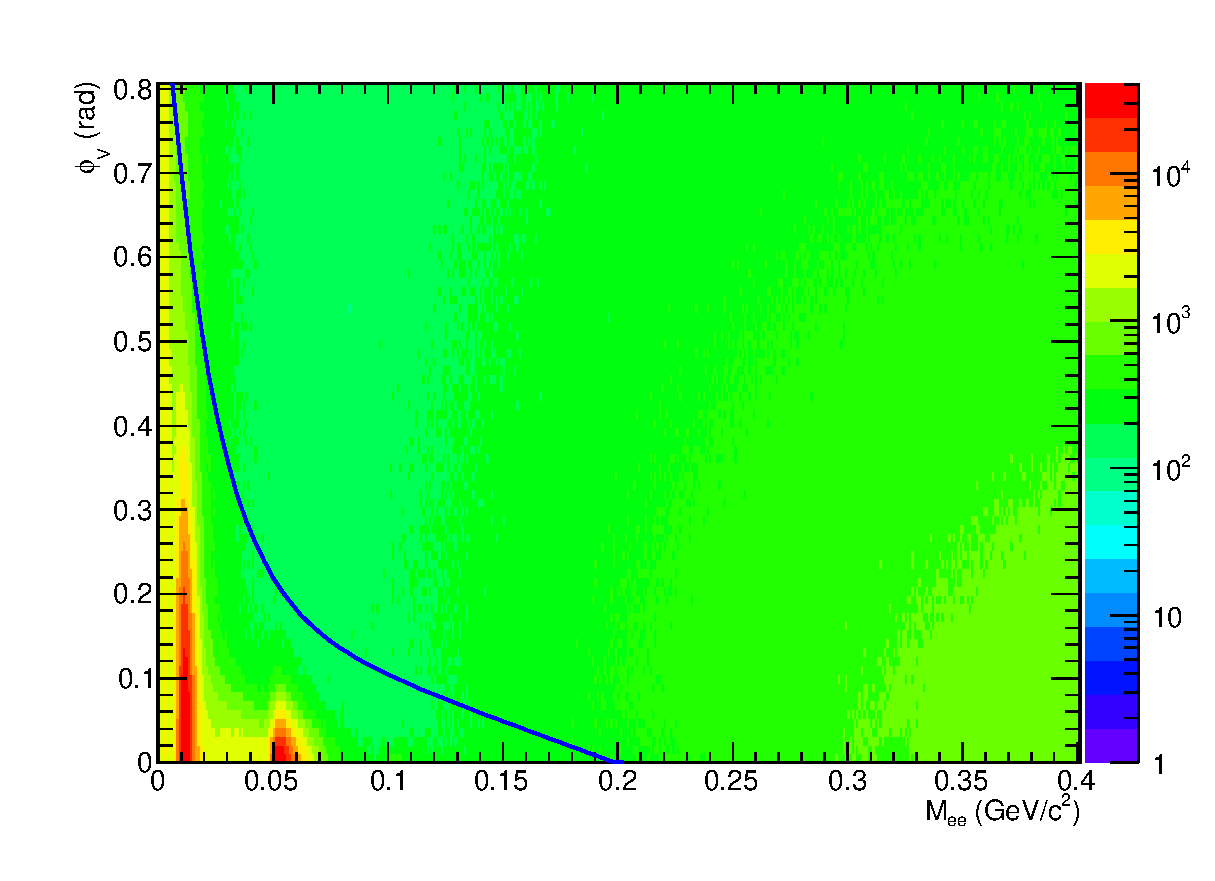
\includegraphics[width=1.0\textwidth]{analysis/sameUnLikeSphiVvsM.eps}
\caption{The $\phi_{V}$ angle vs. invariant mass distribution in Run12 U + U minimum-bias collisions at 193 GeV. The blue solid curve depicts the mass dependent $\phi_{V}$ cut employed to remove the photon conversion electron pairs.\label{phiv:plot}}
\end{minipage}
\hfill
\begin{minipage}[htbp]{0.48\linewidth}
\centering
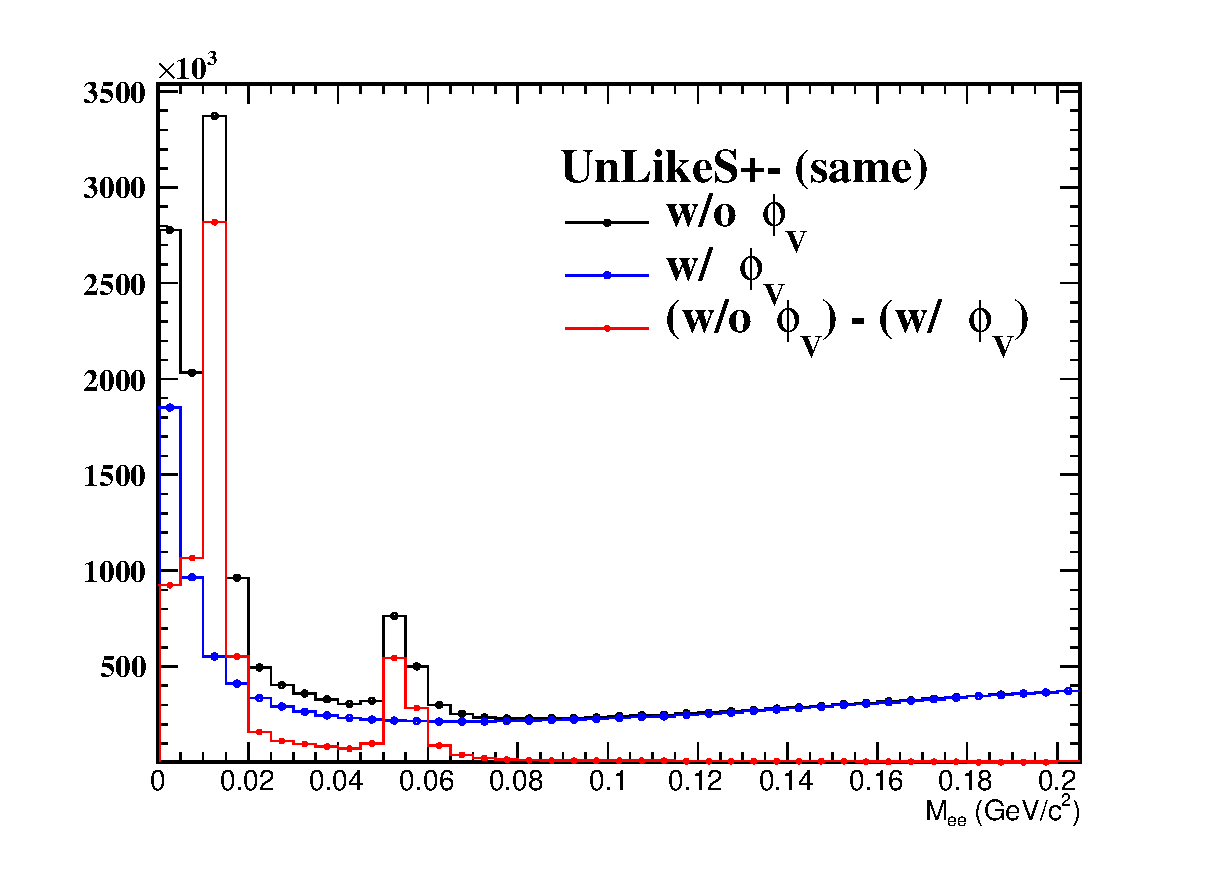
\includegraphics[width=1.0\textwidth]{analysis/gammaConversionE.eps} 
\caption{Red: the invariant mass distribution of the photon conversion electron pairs. Black: the unlike-sign distribution without $\phi_{V}$ cut. Blue: the unlike-sign distribution with $\phi_{V}$ cut.\label{gammaconversion}}
\end{minipage}
\end{figure}

To illustrate the $\phi_{V}$ angle, a little more explanation is added here. Plane A is defined by mother particle momentum direction and beam axis direction, while plane B is defined by the daughter electron, positron momentum directions. The angle between plane A and plane B is defined as $\phi$ ($0^{\circ} \le \phi \le 90^{\circ}$). According to Eq.~\ref{phiv:eq}, $\phi_{V} = 90^{\circ} -/+\;\phi$. For electron and positron from the photon conversion, $\phi = 90^{\circ}$, thus the $\phi_{V}$ angle is zero or $\pi$. A fixed order between electron and positron is used to calculate the $\phi_{V}$ in this analysis for avoiding $\phi_{V} = \pi$ . There is no preferred orientation for combinatorial electron and positron pairs, and only very weak dependence for electron and positron pairs from hadron decays. Figure~\ref{phiv:plot} shows the $\phi_{V}$ angle as a function of invariant mass in U + U minimum-bias collisions at 193 GeV. The blue solid curve depicts the mass dependent $\phi_{V}$ cut employed to remove the photon conversion electron pairs. Figure~\ref{gammaconversion} shows the invariant mass distribution of the photon conversion electron pairs (red curve). As mentioned before, the different invariant mass peak depicts that the conversion electron pairs are from different materials. The mass shifted from zero is because the electrons are assumed to originate from the primary vertex during the final track reconstruction. Therefore, the two main peaks (for the red histogram) from low to high mass correspond to the conversion from the beam pipe and inner cone support structure, respectively.

\subsection{Raw Signal}
The background, in this analysis, is subtracted by the same-event like-sign technique. The same-event like-sign distribution is firstly corrected for the acceptance and then subtracted from the inclusive unlike-sign (foreground) distribution. The invariant mass distribution of signal pairs before detector efficiency losses correction (raw signal) is thus obtained. The upper panel of Fig.~\ref{rawsignal} shows the invariant mass distributions of foreground (black dots), background (black line) and raw signal (blue dots), while the bottom panel shows the signal-to-background ratio in U + U  minimum-bias collisions at $\sqrt{s_{NN}}$ = 193 GeV.

\begin{figure}[htbp]
\centering
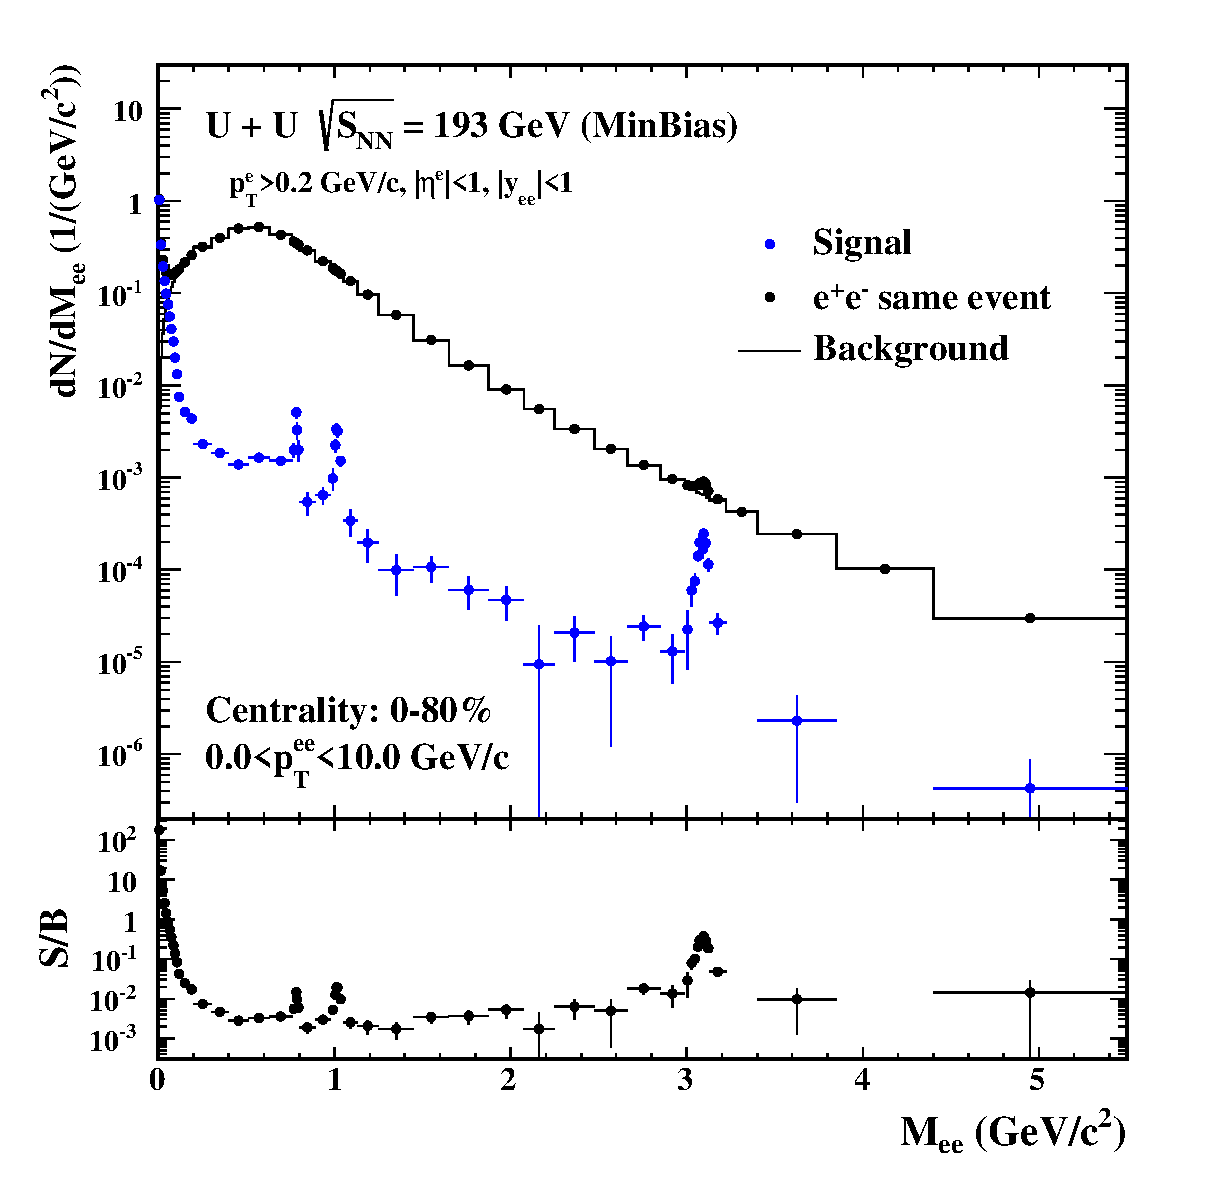
\includegraphics[keepaspectratio,width=0.8\textwidth]{analysis/rawSignal_SBRatio.eps}
\figcaption{(Top) The invariant mass distributions of raw signal (blue dots), foreground (black dots) and background (black line). (Bottom) The signal-to-background ratio in U + U  minimum-bias collisions at $\sqrt{s_{NN}}$ = 193 GeV.}
 \label{rawsignal}
\end{figure}

\section{Efficiency and Acceptance Corrections}
To obtain the real invariant mass spectrum of dielectron within STAR acceptance ($p_{T}^{e} \geq 0.2\;GeV/c, |\eta_{e}| \leq 1, |Y_{ee}| \leq 1$), the raw spectrum should be corrected for the efficiency losses. The pair efficiency within STAR acceptance is evaluated by folding the single track efficiency. To measure the dielectron excess yield and study the medium properties, the dielectron excess spectrum (dielectron invariant mass spectrum with hadronic contributions except $\rho$-meson subtracted, see details in Sec.~\ref{cocktail}) is needed to be corrected for the detector acceptance.

\subsection{Single Track Efficiency}
\label{singletrkeff}
The single track efficiency losses are caused by the detector inefficiency and electron identification cuts. The detector efficiency includes the TPC tracking efficiency ($\varepsilon_{TPC}$), nHitsDedx cut efficiency ($\varepsilon_{nHitsDedx}$) and the TOF matching efficiency ($\varepsilon_{TOF}$). The electron identification cut efficiency ($\varepsilon_{eID}$) includes the efficiencies of TOF velocity and the $dE/dx$ selection cuts. So the single track efficiency can be derived by the Eq.~\ref{singleeff}
\begin{equation}
\varepsilon_{e} = \varepsilon_{TPC} \times \varepsilon_{nHitsDedx} \times \varepsilon_{TOF} \times \varepsilon_{eID}
\label{singleeff}
\end{equation}
Each part will be discussed in the following sub-sections.

\subsubsection{TPC Tracking Efficiency}
\label{embedding}
The TPC tracking efficiency ($\varepsilon_{TPC}$), including the TPC response and acceptance, is evaluated via the standard STAR embedding technique. The Monte Carlo (MC) tracks are embedded into the read data at the raw data level to have a realistic detector occupancy environment. The real data is randomly sampled over the entire U + U minimum-bias data set, while the number of embedded MC tracks is constrained to 5\% of the measured multiplicity of the real events to avoid a sizable impact on the realistic TPC tracking efficiency. The MC tracks, with flat $p_{T}$, $\eta$, and $\phi$, are generated and passed through the full simulation of the STAR detector geometry using the GEANT model~\cite{GEANT}, and then mixed with the real data . The mixed signals are processed using the exactly same off-line reconstruction chain. The quality assurance is made to ensure the MC simulation reproduces the real data before studying the TPC tracking efficiency, The TPC tracking efficiency is derived by taking the ratio of the number of reconstructed MC tracks ($N_{rec}$), satisfying the track quality cuts except nHitsDedx cut used in the data analysis, over the number of embedded MC tracks ($N_{emb}$), as shown in Eq.~\ref{tpceff}
\begin{equation}
\varepsilon_{TPC} = \frac{N_{rec}\;(nHitsFit\geq20\;\&\;\frac{nHitsFit}{nHitsPoss}\geq0.52\;\&\;dca\leq1\;\&\;|\eta|\leq1)}{N_{emb}\;(|\eta|\leq1)}
\label{tpceff}
\end{equation}
The 1-D TPC tracking efficiency in Run12 U + U minimum-bias collisions at 193 GeV is shown in Fig.~\ref{1dtpceff}. However, the 3-D ($p_{T}$, $\eta$, and $\phi$) TPC tracking efficiency will be used in the finally pair efficiency correction, discussed in Sec.~\ref{paireff}.

\subsubsection{nHitsDedx Cut Efficiency}
The nHitsDedx cut efficiency ($\varepsilon_{nHitsDedx}$) is derived from the real data, because the nHitsDedx variable from MC simulation is not consistent with the data. The photonic electron sample (using all track quality and eID cuts except nHitsDedx and the TOF velocity cuts) is selected according to the method discussed in  Sec.~\ref{purity}. The TOF velocity cut is abandoned, because it biases the nHitsDedx to a large number due to the TOF matching algorithm. The nHitsDedx cut efficiency is then derived by comparing the number of photonic electron tracks with and without nHitsDedx cut. Figure~\ref{nhitsdedxeff} shows the nHitsDedx cut efficiency as a function of $p_{T}$ in Run12 U + U minimum-bias collisions at 193 GeV.

\begin{figure}[htbp]
\begin{minipage}[htbp]{0.48\linewidth}
\centering
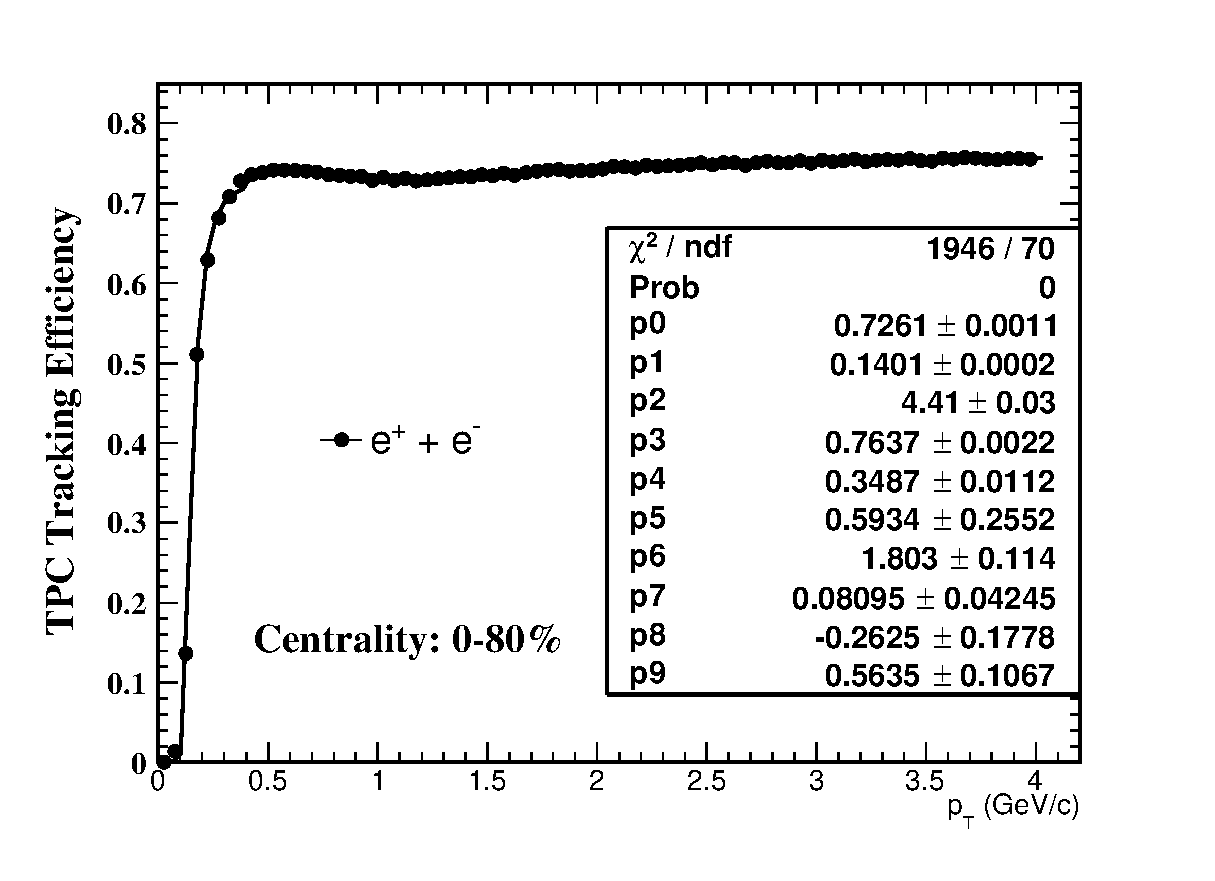
\includegraphics[width=1.0\textwidth]{analysis/TpcEff_MB.eps}
\caption{The 1-D TPC tracking efficiency in Run12 U + U minimum-bias collisions at 193 GeV.\label{1dtpceff}}
\end{minipage}
\hfill
\begin{minipage}[htbp]{0.48\linewidth}
\centering
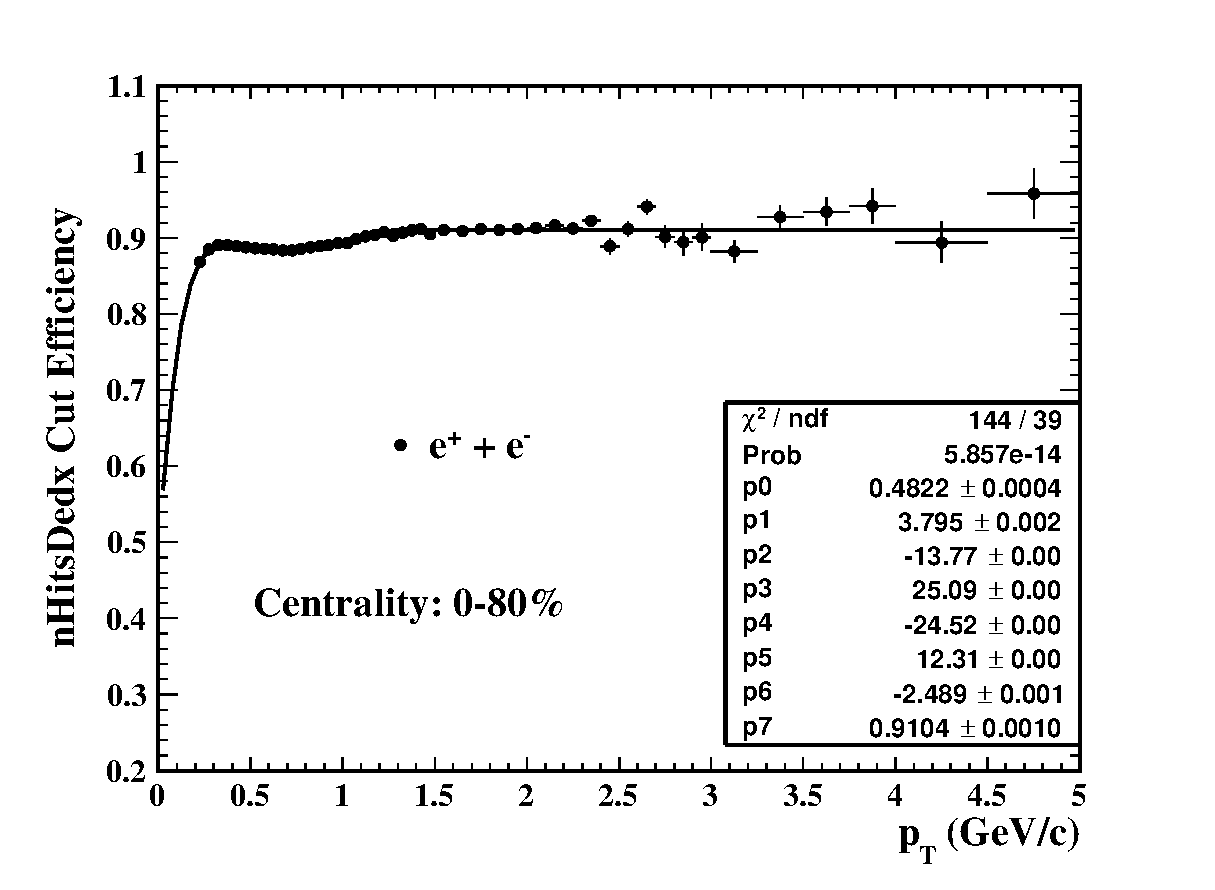
\includegraphics[width=1.0\textwidth]{analysis/PHE_nHitsDedxEff.eps} 
\caption{The nHitsDedx cut efficiency in Run12 U + U minimum-bias collisions at 193 GeV.\label{nhitsdedxeff}}
\end{minipage}
\end{figure}

\subsubsection{TOF Matching Efficiency}
The TOF matching efficiency ($\varepsilon_{TOF}$), including the TOF response and the acceptance difference between the TPC and TOF, is evaluated by the real data. It can be calculated by comparing the number of qualified primary tracks matched with the TOF (with $\beta$ > 0, $N_{matched}$) over  the number of qualified primary tracks ($N_{TPC}$). Due to the limited statistics of  pure electron sample, the pure pion sample selected by a tight TPC $dE/dx$ cut (|$n\sigma_{\pi}$| < 0.6), is thus used to generate the 3-D ($p_{T}$, $\eta$, and $\phi$) TOF matching efficiency. The TOF matching efficiency difference between the electron and pion is then corrected for each ($\eta$, $\phi$) bin using the same $p_{T}$ dependent correction factor. The TOF matching efficiency difference between electrons and pions, is due to the decay loss of pions between the TPC and TOF as well as other effects (e.g. pile-up effect). The 1-D TOF matching efficiency and the $p_{T}$ dependent correction factor are shown in Fig.~\ref{tofeff}.

\begin{figure}[htbp]
\centering
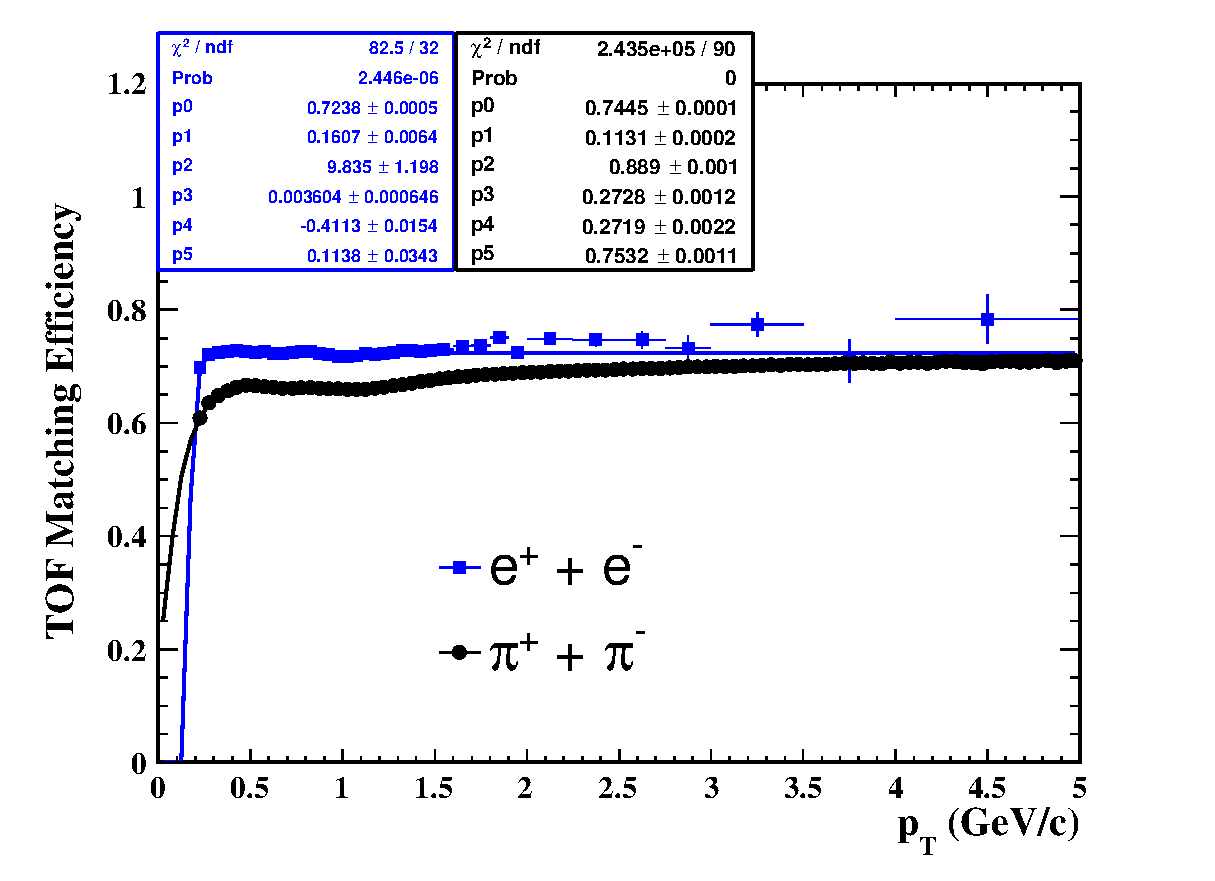
\includegraphics[width=0.48\textwidth]{analysis/PHE_Pion_TofEff.eps}
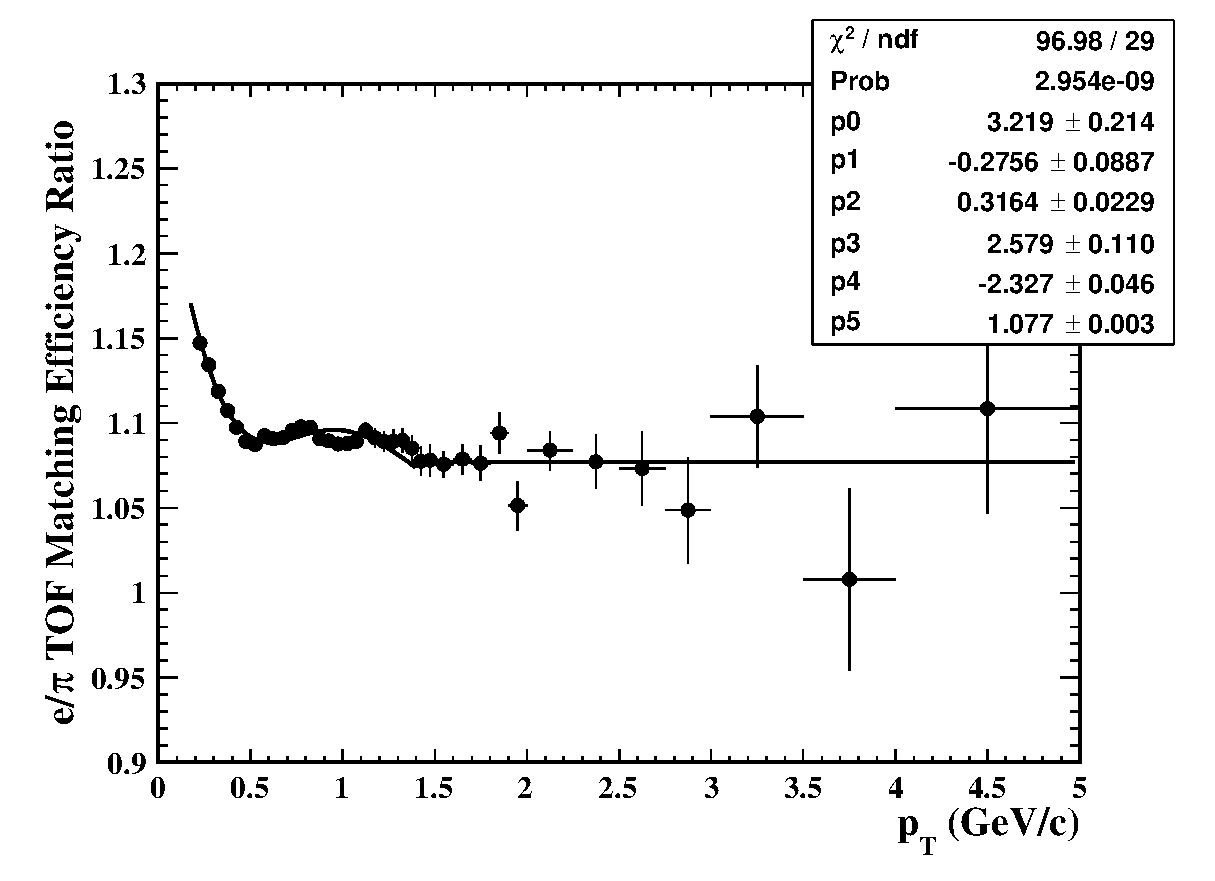
\includegraphics[width=0.48\textwidth]{analysis/PHE_Pion_TofEffRatio.eps}
\figcaption{(Left) The 1-D TOF matching efficiency for pure electron and pion sample in Run12 U + U minimum-bias collisions at 193 GeV. (Right) The corresponding TOF matching efficiency ratio of electron over pion as a function of $p_{T}$.}
\label{tofeff}
\end{figure}

\subsubsection{eID Cuts Efficiency}
\label{eideff}
The electron identification cut efficiency ($\varepsilon_{eID}$) includes two components: the TOF velocity ($1/\beta$) cut efficiency and $dE/dx$ cut ($n\sigma_{e}$) efficiency. Pure electron sample is used to evaluate the TOF velocity cut efficiency, and the $1/\beta$ distribution of the pure electron is shown in the left panel of Fig.~\ref{betaeff}. The red lines depict the $1/\beta$ cut used in this analysis, and the efficiency is calculated using two methods: a Gaussian fit the $1/\beta$ distribution and direct counting for each $p_{T}$ bin. The Gaussian fit overestimates the $1/\beta$ cut efficiency due to the tail structure in each $p_{T}$ bin. Thus the default $1/\beta$ cut efficiency value, shown in the right panel (blue circles) of Fig.~\ref{betaeff}, comes from the direct counting method, and the difference between this two methods is taken into account for the systematic uncertainty. The $n\sigma_{e}$ cut efficiency is derived from the multi-Gaussian fit discussed in Sec.~\ref{purity}. Figure~\ref{nsigmaeeff} depicts the $n\sigma_{e}$ cut efficiency in Run12 U + U minimum-bias collisions at 193 GeV.

\begin{figure}[htbp]
\centering
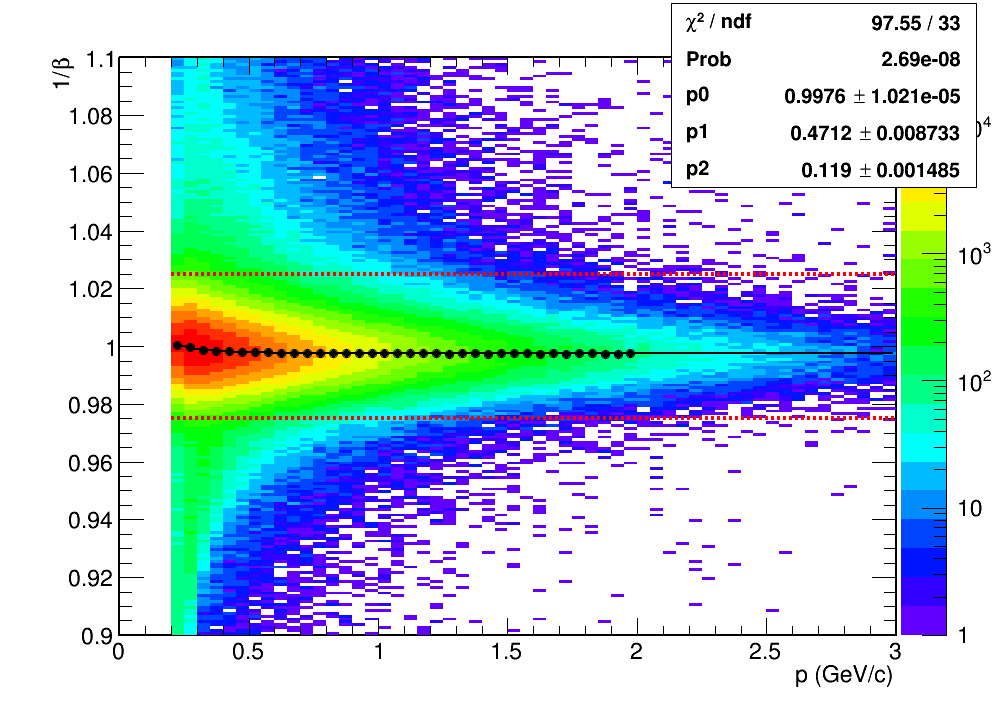
\includegraphics[width=0.48\textwidth]{analysis/PHE_beta.png}
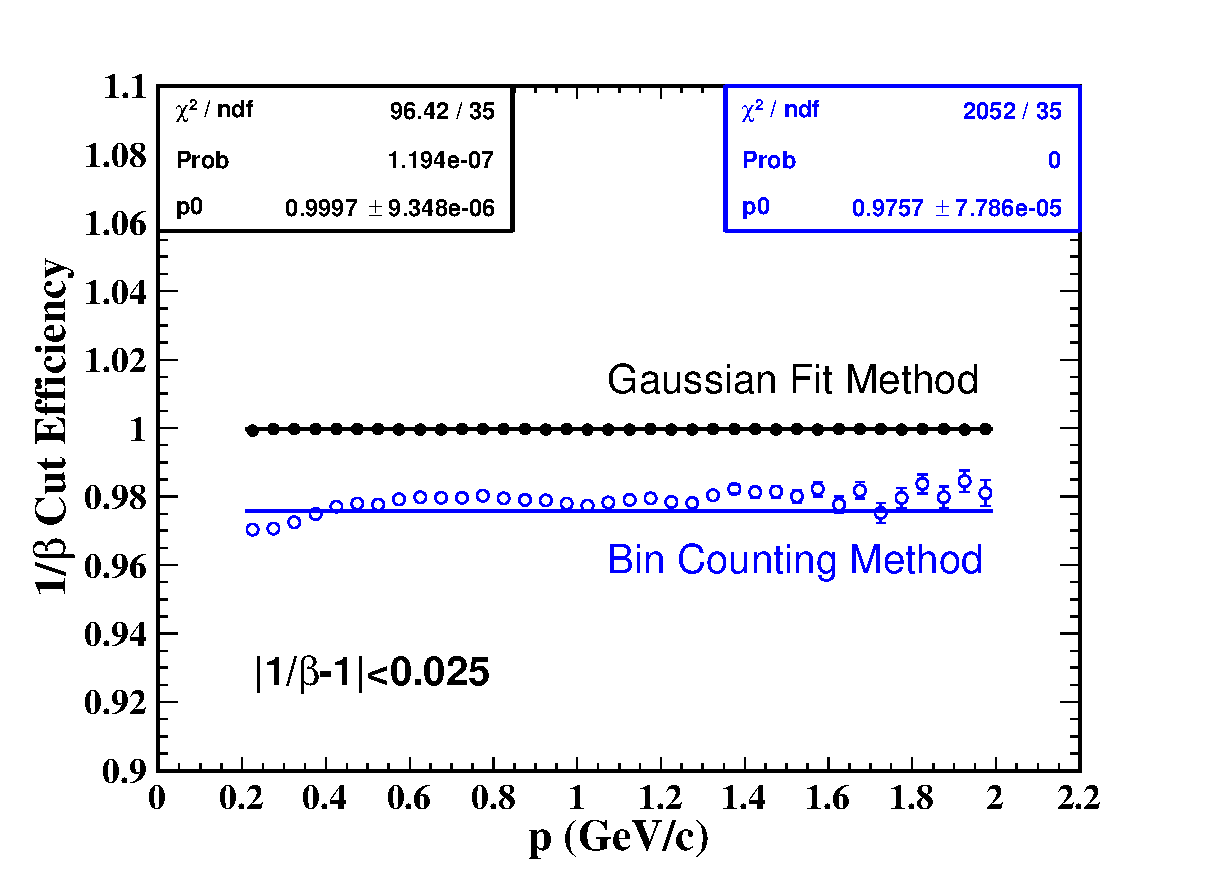
\includegraphics[width=0.48\textwidth]{analysis/Beta_CutEff_Minus1.eps}
\figcaption{(Left) The $1/\beta$ distribution for pure electron sample in Run12 U + U minimum-bias collisions at 193 GeV. Red dashed lines represent the $1/\beta$ cut used in this analysis. Black dots represent the $1/\beta_{mean}$ for each $p_{T}$ bin while the black curve is the fit function. (Right) The $1/\beta$ cut efficiencies using bin counting (default, blue circles) and Gaussian fit (black dots) methods.}
\label{betaeff}
\end{figure}

\begin{figure}[htbp]
\centering
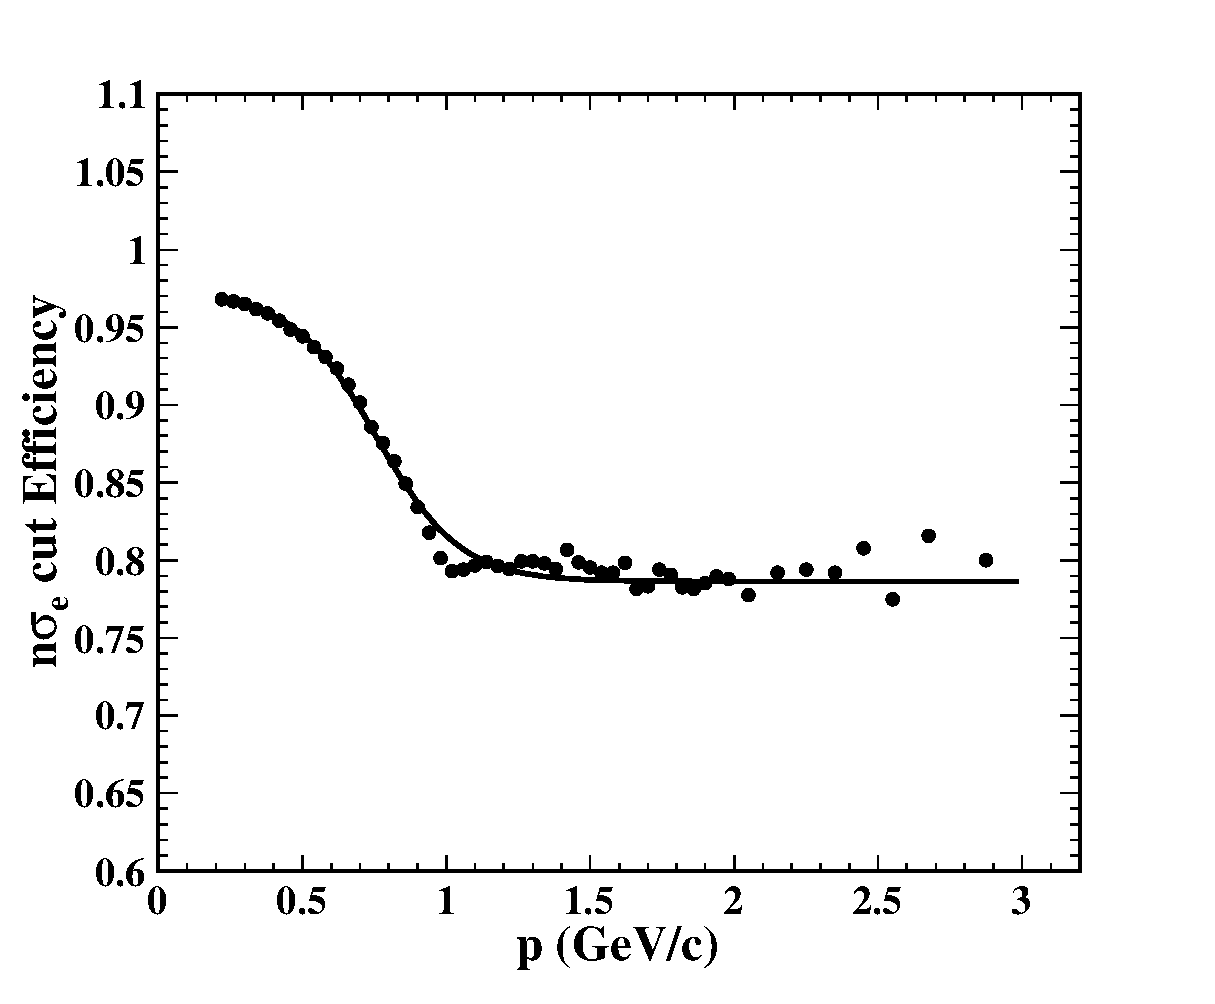
\includegraphics[keepaspectratio,width=0.6\textwidth]{analysis/nSigEcut4TpcE_Eff.eps}
\figcaption{The $n\sigma_{e}$ cut efficiency in U + U  minimum-bias collisions at 193 GeV.}
 \label{nsigmaeeff}
\end{figure}

\subsection{Pair Efficiency and Acceptance}
\label{paireff}

\paragraph{Pair Efficiency}
The dielectron pair efficiency within STAR acceptance ($p_{T}^{e}$ $\geq$ 0.2 GeV/$c$, $|\eta_{e}|$ $\leq$ 1, $|Y_{ee}|$ $\leq$ 1) is evaluated from single track efficiency by two different simulation folding methods:
\begin{itemize}
\item[(i)] Toy MC simulation (Virtual photon simulation), which uses the virtual photon as input. The 2-D kinematics ($M_{ee}, p_{T}$) of the virtual photon is taken from the hadronic cocktail (discussed in Sec.~\ref{cocktail}) with flat rapidity (Y), azimuthal ($\phi$) distribution, and the virtual photon decays into electron and positron pairs isotropically.
\item[(ii)] Cocktail simulation, which uses the hadronic cocktail as input, including the correlated heavy flavor decay ($c\overline{c}$, $b\overline{b}$) and Drell-Yan process from PYTHIA~\cite{Pythia} simulation. The long-lived hadrons decay into electron and positron pairs isotropically. However, the electron and position from the heavy flavor decay are highly correlated.
\end{itemize} 
The largest difference between these two methods is the correlated heavy flavor contribution, which is still unclear in heavy-ion collisions due to possible medium modifications of the heavy flavor correlations compared to those in $p$ + $p$ collisions. In this analysis, the heavy flavor correlations rely on the PYTHIA simulation without any artificial modification.

The single track efficiencies caused by the TPC tracking and TOF matching are folded into pair efficiency in 3-D ($p_{T}$, $\eta$, and $\phi$) momentum space while the others are folded in 1-D ($p_{T}$) momentum space. The momentum resolution and energy loss effects, discussed in Sec.~\ref{cocktail}, are also taken into account during the folding process. The pair efficiency is calculated and applied in 2-D kinematics ($M_{ee}, p_{T}$). Figure~\ref{paireff2d} shows the 2-D pair efficiency evaluated by the ``Virtual photon simulation'' and ``Cocktail simulation'' methods in Run12 U + U minimum-bias collisions at 193 GeV. Figure~\ref{paireff1d} shows the 1-D pair efficiency comparisons between these two methods, and the differences are pretty small. The default pair efficiency is evaluated by the ``Virtual photon simulation'' and the difference between these two methods is taken into account for systematic uncertainty.  

\begin{figure}[htbp]
\centering
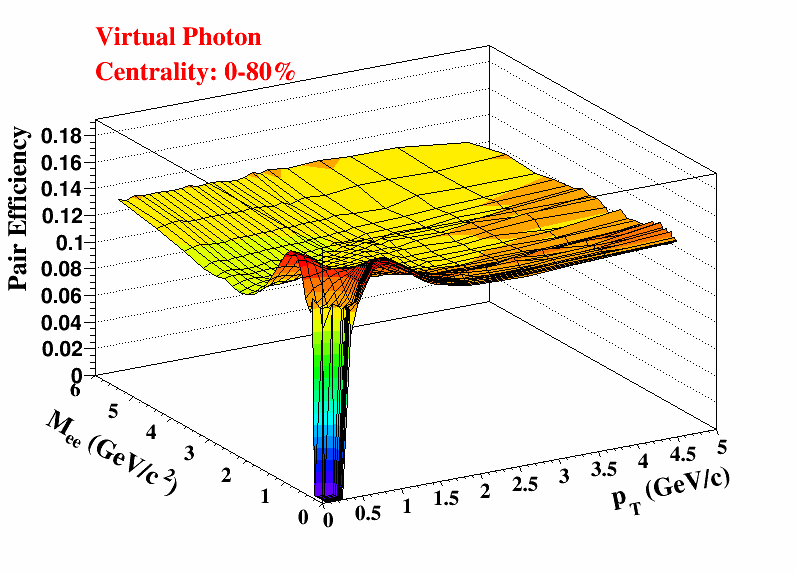
\includegraphics[width=0.48\textwidth]{analysis/pairEff2D_VP_Cen0_80.png}
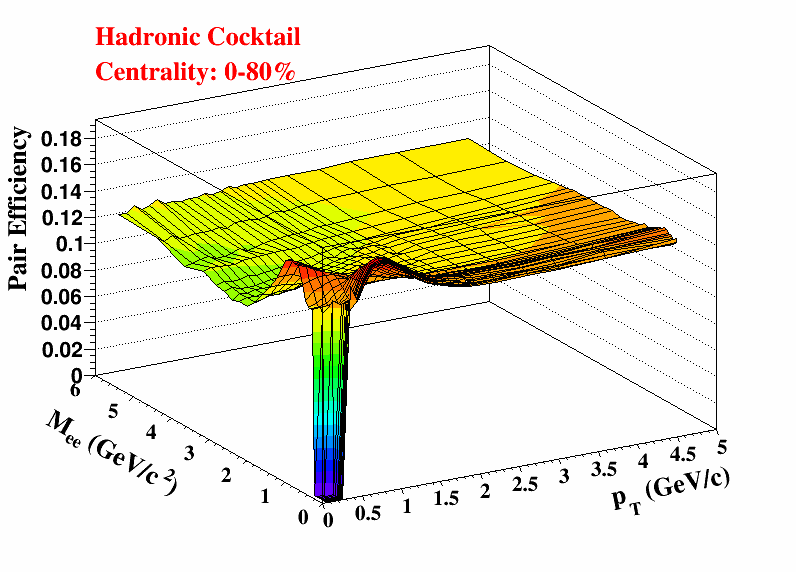
\includegraphics[width=0.48\textwidth]{analysis/pairEff2D_Cock_Cen0_80.png}
\figcaption{The 2-D pair efficiency evaluated by the ``Virtual photon simulation'' (Left) and ``Cocktail simulation'' (Right) methods in Run12 U + U minimum-bias collisions at 193 GeV.}
\label{paireff2d}
\end{figure}

\begin{figure}[htbp]
\centering
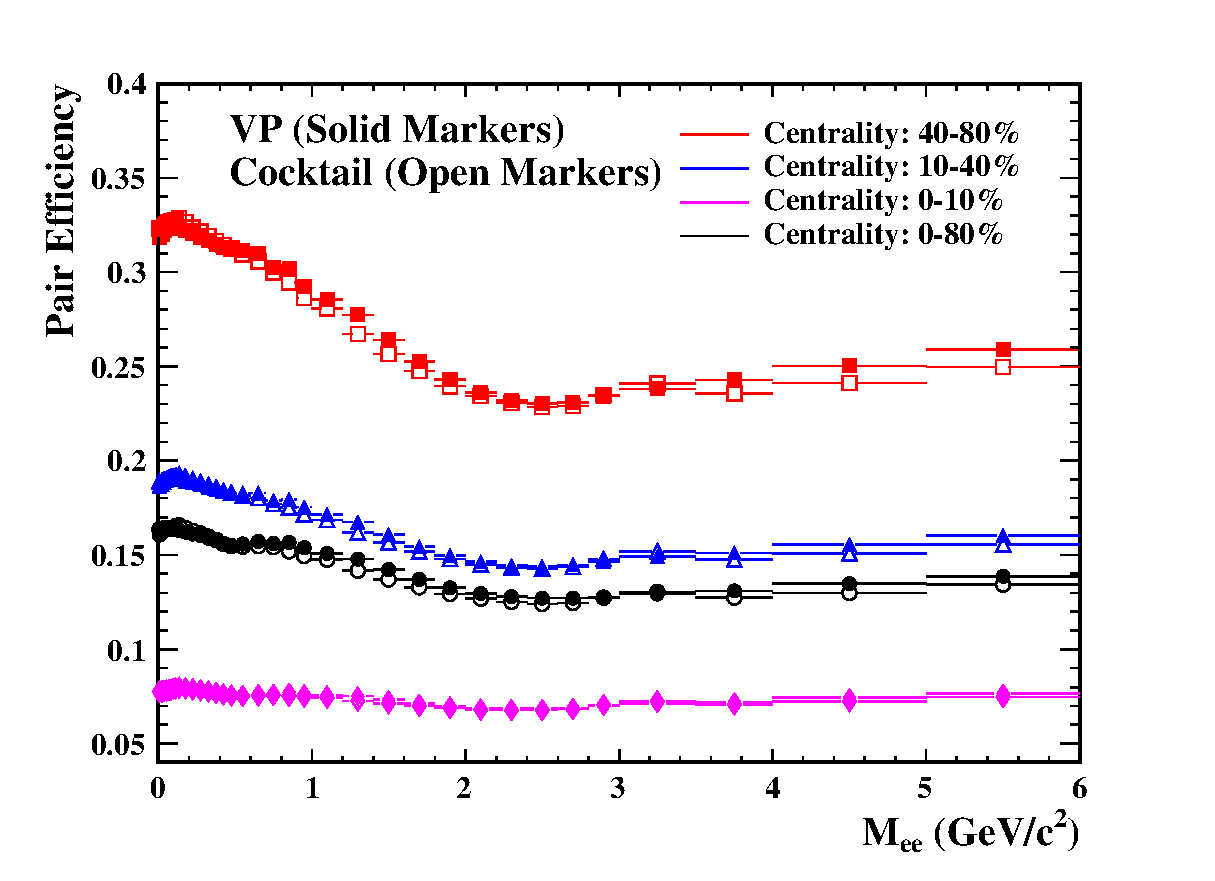
\includegraphics[keepaspectratio,width=0.6\textwidth]{analysis/pairEff1D_AllCens.eps}
\figcaption{The 1-D pair efficiency comparisons between the ``Virtual photon simulation'' (Solid Markers) and ``Cocktail simulation'' (Open Markers) for different centralities in Run12 U + U collisions at 193 GeV.}
 \label{paireff1d}
\end{figure}

The $\phi_{V}$ cut (reject electron pairs) efficiency is evaluated through $\pi^{0}$ Dalitz decay embedding (see Sec.~\ref{embedding}) and the virtual photon simulation. The $\phi_{V}$ cut efficiency obtained by these two methods is shown in Fig.~\ref{phiveff}. The default $\phi_{V}$ cut efficiency is evaluated by the virtual photon simulation and the difference between these two methods is taken into account for the systematic uncertainty.

\begin{figure}[htbp]
\centering
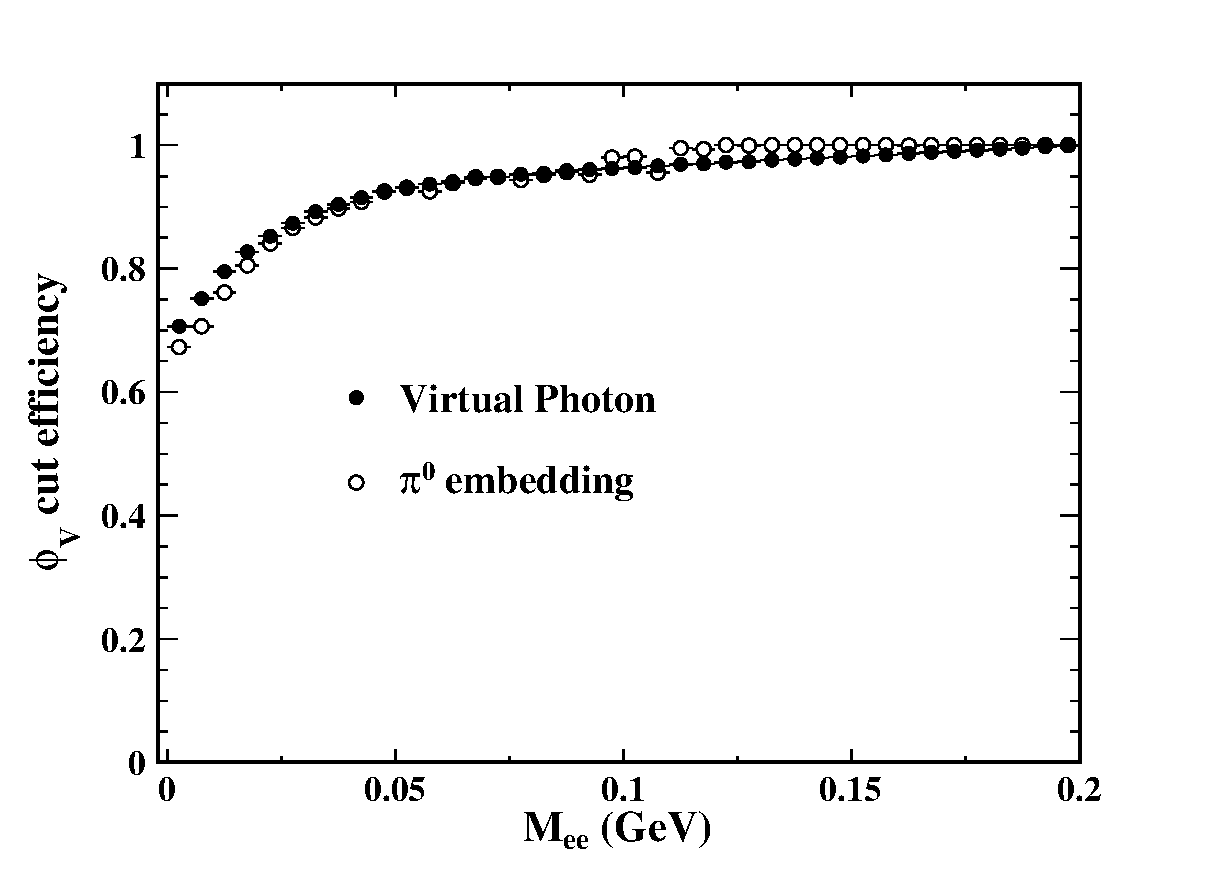
\includegraphics[keepaspectratio,width=0.6\textwidth]{analysis/phiV_eff.eps}
\figcaption{The $\phi_{V}$ angle cut efficiencies obtained by $\pi^{0}$ Dalitz decay embedding and virtual photon simulation.}
 \label{phiveff}
\end{figure}

\begin{figure}[htbp]
\centering
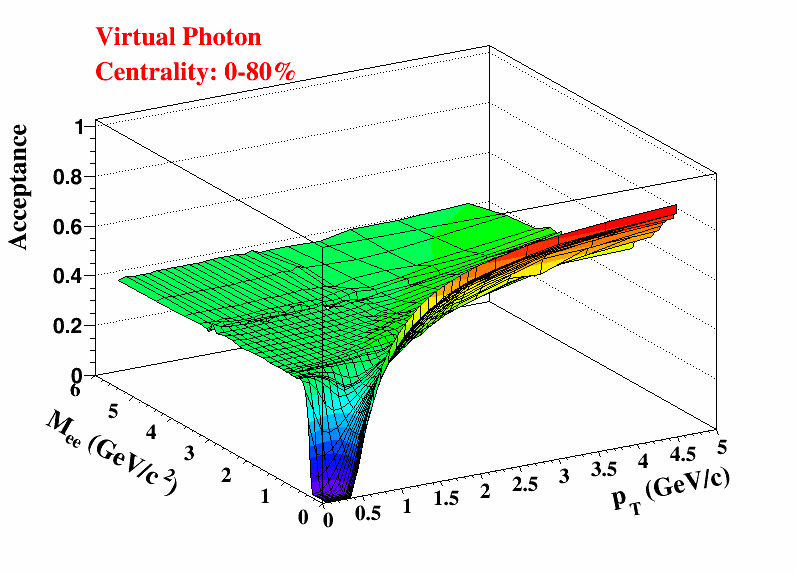
\includegraphics[width=0.48\textwidth]{analysis/Acceptance2D_VP_Cen0_80.png}
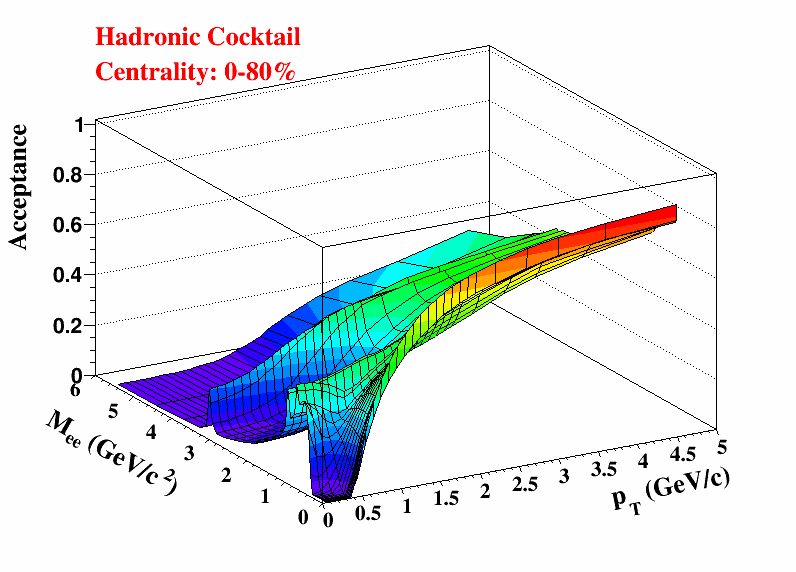
\includegraphics[width=0.48\textwidth]{analysis/Acceptance2D_Cock_Cen0_80.png}
\figcaption{The 2-D detector acceptance derived by the ``Virtual photon simulation'' (Left) and ``Cocktail simulation'' (Right) methods in Run12 U + U minimum-bias collisions at 193 GeV.}
\label{acceptance2d}
\end{figure}

\begin{figure}[htbp]
\centering
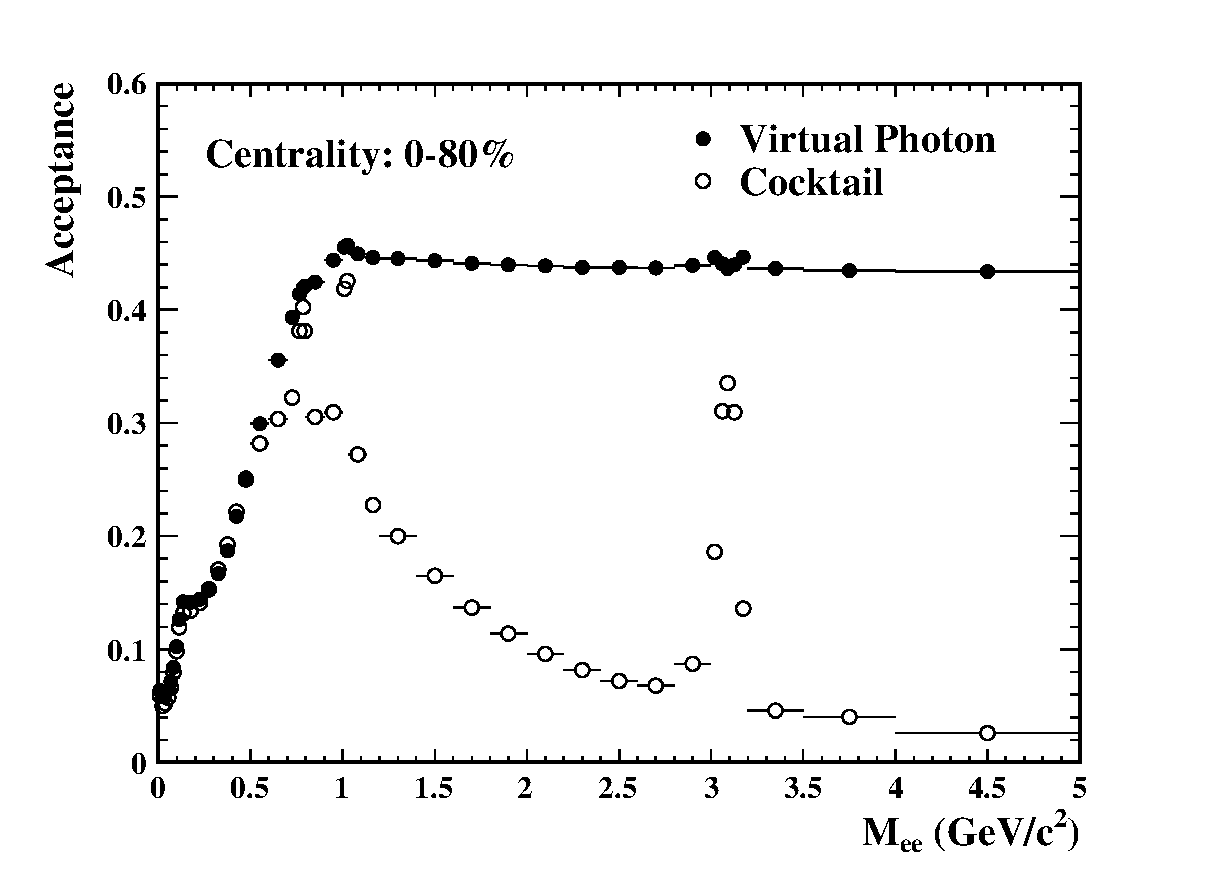
\includegraphics[keepaspectratio,width=0.6\textwidth]{analysis/Acceptance1D_MB.eps}
\figcaption{The 1-D detector acceptance comparison between the ``Virtual photon simulation'' and ``Cocktail simulation'' in Run12 U + U minimum-bias collisions at 193 GeV.}
 \label{acceptance1d}
\end{figure}

\paragraph{Acceptance}
The efficiency-corrected dielectron spectrum is within STAR acceptance ($p_{T}^{e} \geq 0.2\;GeV/c, |\eta_{e}| \leq 1, |Y_{ee}| \leq 1$). Thus the dielectron excess spectrum (dielectron invariant mass spectrum with hadronic contributions except $\rho$-meson removed. See details in Sec.~\ref{cocktail}) is needed to be corrected for the detector acceptance to quantitatively measure the excess yields and study the medium properties. The acceptance factor is calculated by taking the ratio of dielectron yields after over before filtering STAR acceptance, as shown in the following equation:
\begin{equation}
\varepsilon_{Acc} = \frac{dN/dM_{ee}\;(p_{T}^{e}\geq0.2\;GeV/c\;,\;|\eta_{e}|\leq1\;,\;|Y_{ee}|\leq1)}{dN/dM_{ee}\;(|Y_{ee}|\leq1)}
\label{acceptance:eq}
\end{equation}
The acceptance correction can be evaluated using the same methods (``Virtual photon simulation'', ``Cocktail simulation'' ) described in the pair efficiency correction section. However, the acceptance factors evaluated by these two methods have a huge difference in the IMR, as shown in Fig.~\ref{acceptance2d} and Fig.~\ref{acceptance1d}. The difference is due to the unknown charm correlation which dominates in the dielectron IMR at RHIC energy. In IMR, the correlation of electron pairs is from the pure decay kinematics in the ``Virtual photon simulation'' method while that inherits the correlation of strong correlated charm generated by PYTHIA in ``Cocktail simulation'' method. The acceptance factor evaluated by the ``Virtual photon simulation'' method is finally applied to the excess spectrum, which does not contain the heavy flavor contribution, in 2-D kinematics ($M_{ee}$, $p_{T}$).

\section{Hadronic Cocktail Simulation}
\label{cocktail}
Dielectrons as measured by the detector originate from all stage in the evolution of heavy-ion collisions. The contribution of the dielectron pairs from hadronic decays, so called hadronic cocktail, to the final dielectron spectrum can be well evaluated trough MC simulation once their yields and $p_{T}$ spectra are measured. The components of the cocktail simulation in this analysis are listed below:
\begin{itemize}
\item[(i)] Two-body decays: $\omega \rightarrow e^{+}e^{-}$, $\phi \rightarrow e^{+}e^{-}$, $J/\psi \rightarrow e^{+}e^{-}$, $\psi^{\prime} \rightarrow e^{+}e^{-}$.
\item[(ii)] Dalitz decays: $\pi^{0} \rightarrow \gamma e^{+}e^{-}$, $\eta \rightarrow \gamma e^{+}e^{-}$, $\eta^{\prime} \rightarrow \gamma e^{+}e^{-}$, $\omega \rightarrow \pi^{0}e^{+}e^{-}$, $\phi \rightarrow \eta e^{+}e^{-}$.
\item[(iii)] Heavy-flavor decays: $c\overline{c} \rightarrow e^{+}e^{-}+X$, $b\overline{b} \rightarrow e^{+}e^{-}+X$.
\item[(iv)] Drell-Yan process.
\end{itemize}
The $\rho^{0}$, considered to be modified by the hadronic medium, is excluded in the cocktail simulation. 

For U + U collisions at 193 GeV, there is no measurement for the identified particle species. However, the energy density created in U + U collisions at $\sqrt{s_{NN}}$ = 193 GeV is only about 20\% higher than that in Au + Au collisions at $\sqrt{s_{NN}}$ = 200 GeV~\cite{UUEnergyDensity}. Thus the hadron $p_{T}$ spectra in Au + Au collisions at 200 GeV~\cite{STAR:dielectron1} are employed for cocktail simulation in this analysis, as shown in Fig.~\ref{tbwfit}. The measurements of identified particle species (the symbols in Fig.~\ref{tbwfit}) except $J/\psi$ in Au + Au collisions at 200 GeV, are simultaneously fitted by a core-corona-based Tsallis Blast-Wave (TBW) model~\cite{TBW0, TBW1}. The core and corona describe the bulk production and the hard scattering contributions from $p$ + $p$-like collisions, respectively. The $J/\psi$ is excluded from simultaneously fit, because the $J/\psi$ is not considered as a component of the bulk medium. The TBW fit can well describe the measured light hadron spectra and also provide predictions for the meson species without measurement (e.g. low $p_{T}$ $\eta$, $\eta^{\prime}$, $\omega$) using the same core TBW parameters obtained from the simultaneously fit. The rapidity and azimuthal distribution of the input hadron are assumed to be flat. The yields ($dN/dy$) of the input hadron in Au + Au collisions are extracted  by integrating the fits over the whole $p_{T}$ region.

\begin{figure}[htbp]
\centering
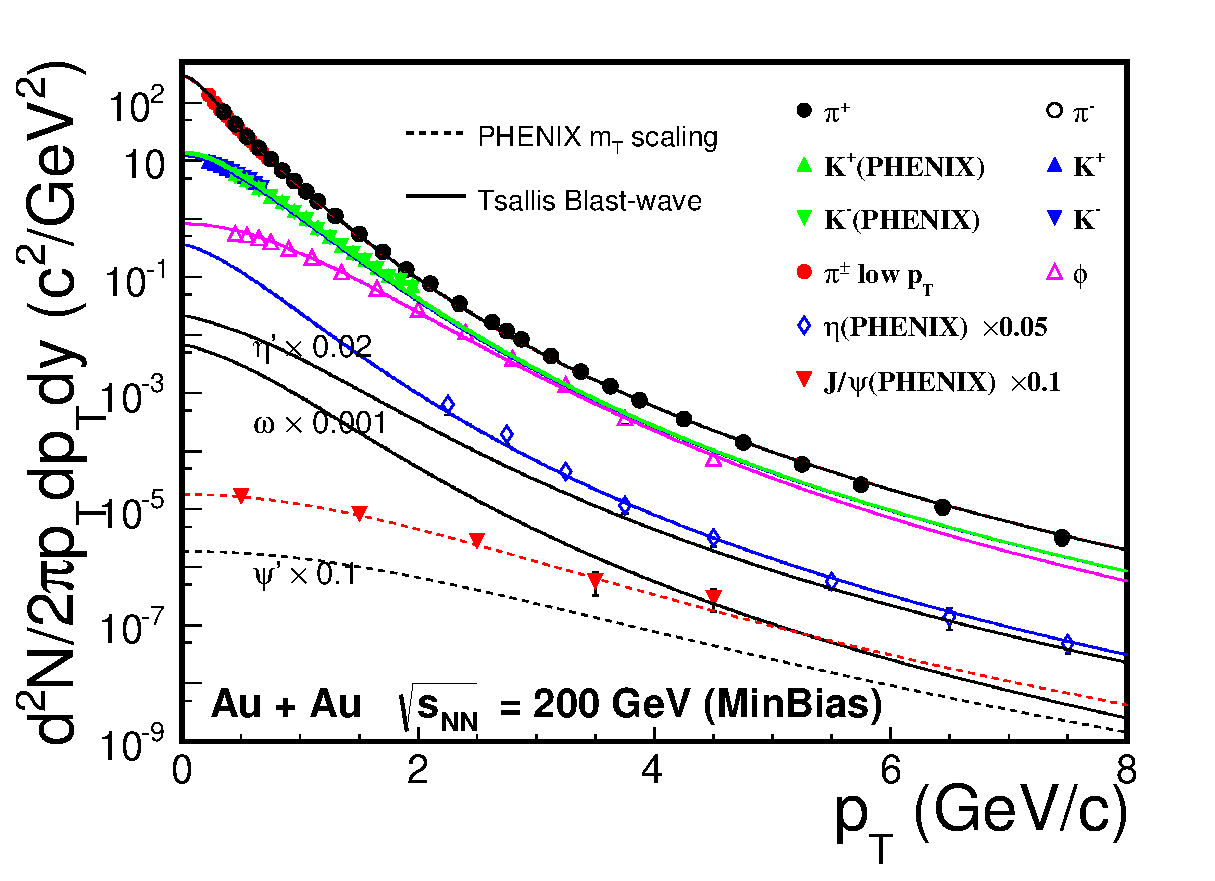
\includegraphics[keepaspectratio,width=0.6\textwidth]{analysis/TBW_AuAu200GeV.eps}
\figcaption{The invariant yields of mesons in Au + Au collisions at 200 GeV. The solid lines show the simultaneous TBW fit to the measured data points (except J/$\psi$) and the TBW predictions for $\eta$, $\eta^{\prime}$, and $\omega$ with the same core TBW parameters. The dashed lines show the TBW fit to the measured J/$\psi$ and the prediction for the $\psi^{\prime}$.}
 \label{tbwfit}
\end{figure}

The $dN/dy$ or cross section ($\sigma$) with their uncertainties and corresponding decay branching ratios of various cocktail components used in Au + Au minimum-bias collisions at 200 GeV, are summarized in~\cite{STAR:dielectron1} (TABLE \uppercase\expandafter{\romannumeral3}). The $dN/dy$ of cocktail hadron components (without measurements) used in U + U minimum-bias collisions at 193 GeV are essentially derived from that of Au + Au minimum-bias collision at 200 GeV by $N_{part}$. The $\pi^{0}$ $dN/dy$ (($\pi^{+} + \pi^{-}$)/2)~\cite{IdentPartYieldsPRCLong} of Au + Au collisions at 200 GeV scaled by $N_{part}/2$ as a function of $N_{part}$, is fitted by a first-order polynomial function. The $\pi^{0}$ $dN/dy$ of U + U collisions at 193 GeV for different centralities are evaluated by this first-order polynomial function, as shown in Fig.~\ref{uupi0yields}. The input $dN/dy$ for other cocktail hadron components (except $J/\psi$ and $\psi^{\prime}$) in U + U minimum-bias collisions at 193 GeV are scaled with the relative pion yields, $R_{\pi^{0}}$ (shown in Tab.~\ref{uupi0}), with respect to Au + Au minimum-bis collisions at 200 GeV. The $dN/dy$ of $J/\psi$ and $\psi^{\prime}$ are scaled by relative $N_{coll}$. The quoted systematic uncertainties of the hadron yields are the same as that of Au + Au collisions at 200 GeV. The input $p_{T}$ spectra of cocktail hadron components for different centralities in U + U collisions at 193 GeV, are also the same as those (using the similar TBW function fit to the available data) of the corresponding centralities in Au + Au collisions at 200 GeV. The heavy flavor contributions to the hadronic cocktail will be discussed later.

\begin{figure}[htbp]
\centering
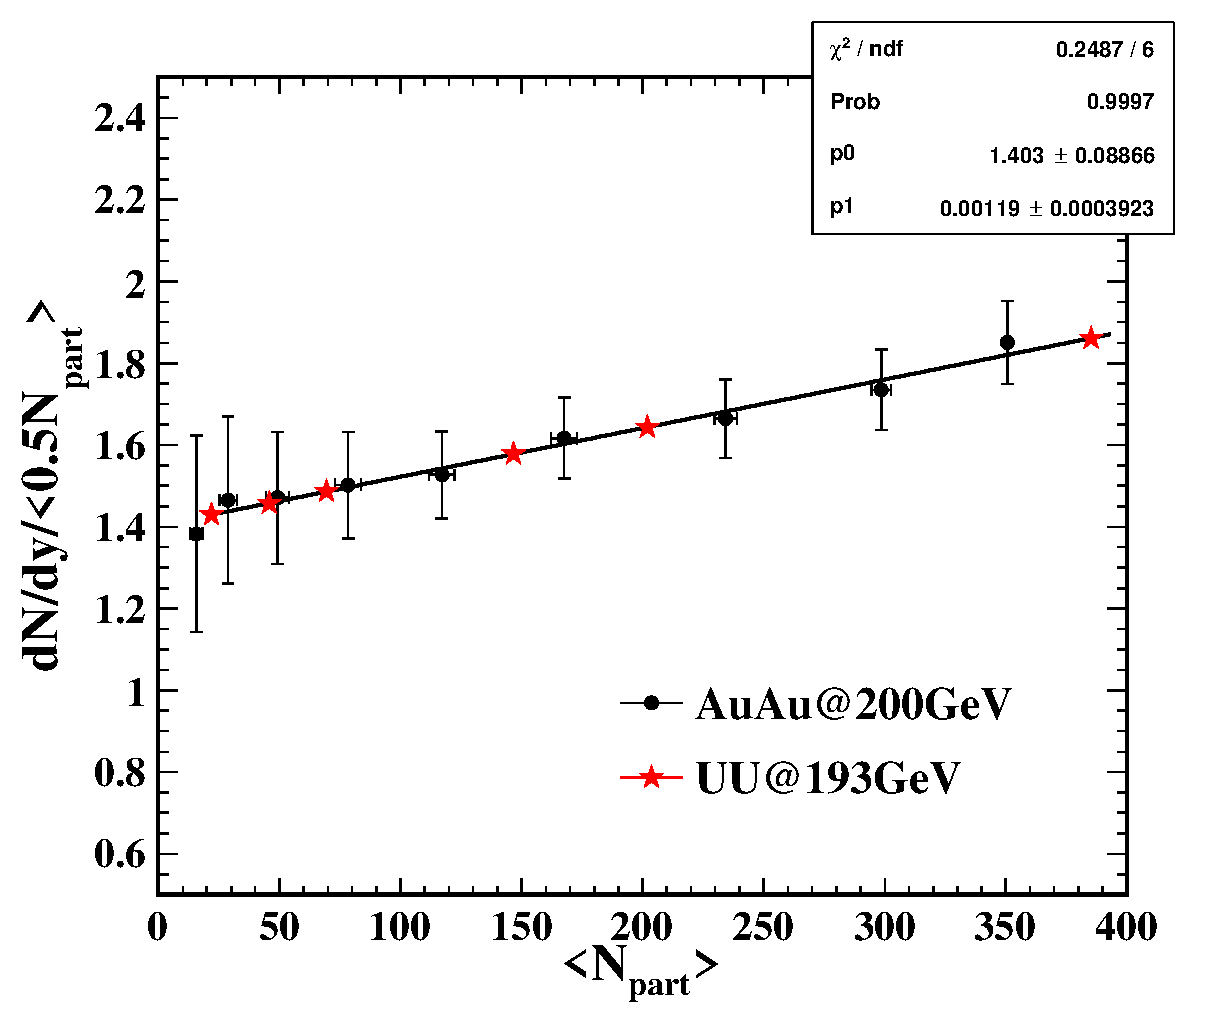
\includegraphics[keepaspectratio,width=0.6\textwidth]{analysis/AuAuUU_normalized_pi0dNdy_vs_Npart.eps}
\figcaption{The $\pi^{0}$ yields (black dots) scaled by $N_{part}/2$ as a function of $N_{part}$ is fitted by a first-order polynomial function (black line).  The $\pi^{0}$ yields of U + U collisions for different centralities (red stars) are evaluated by this fit function.}
 \label{uupi0yields}
\end{figure}

\begin{table}[htp]
\centering
\caption{The scale factors ($R_{\pi^{0}}$) for different centralities in U + U collisions at 193 GeV, with respect to the $dN_{\pi^{0}}/dy$ (98.49) Au + Au minimum-bias collisions at 200 GeV.}
\label{uupi0}
\begin{tabular}{lr@{.}lr@{.}lr@{.}l}
\Xhline{1.6pt}
Centrality (\%) & \multicolumn{2}{c}{$dN_{\pi^{0}}/dy$} & \multicolumn{2}{c}{$R_{\pi^{0}}$} & \multicolumn{2}{c}{$\langle$$N_{coll}$$\rangle$} \\
\Xhline{1.2pt}
 0-80 & 115&76 & 1&175 & 350&08 \\
 60-80 & 15&72 & 0&160 & 22&48  \\
 40-80 & 33&35 & 0&339 & 63&05  \\
 40-60 & 51&65 & 0&524 & 103&61 \\
 10-40 & 165&90 & 1&684 & 467&44 \\
 0-10 & 358&48 & 3&640 & 1146&12 \\
\Xhline{1.6pt}
\end{tabular}
\end{table}

Once the kinematics ($p_{T}$, $\eta$, and $\phi$) of the parent hadron obtained, the kinematics of the daughter electrons are determined by the decay kinematics. The electron pair mass depends on the parent particle and the decay mode (two-body decay or Dalitz decay). The electron pair mass of two-body decay follows a narrow Breit-Wigner distribution as given in Eq.~\ref{breit:wigner}
\begin{equation}
\frac{dN}{dM_{ee}} = \frac{2\Gamma_{0}}{(M_{ee} - M_{h})^{2} + \Gamma_{0}^{2}/4}
\label{breit:wigner}
\end{equation}
where the $\Gamma_{0}$ represents the PDG~\cite{PDG} width, and $M_{h}$ is the mass of the hadron which decays into the dielectron. The electron pair mass ($M_{ee}$) is constrained to [$2m_{e}$, 4 $GeV/c^{2}$], where the $m_{e}$ is the electron mass. The electron pair mass of Dalitz decay follows the Kroll-Wada formula~\cite{KrollWada} as given in Eq.~\ref{kroll:wada}, 
\begin{equation}
\frac{dN}{dM_{ee}} = PS \cdot |F(M_{ee}^{2})|^{2} \cdot QED
\label{kroll:wada}
\end{equation}
Where PS is the phase space term defined in Eq.~\ref{ps:com}. The $M_{h}$ is mass of the hadron which undergoes a Dalitz decay process ($h \rightarrow Xe^{+}e^{-}$) and $X$ is the third daughter particle with a mass $M_{X}$. if $X$ is massless (e.g. $\gamma$ in $\pi^{0}$, $\eta$, $\eta^{\prime}$ Dalitz decay), the phase space term simplifies to Eq.~\ref{ps:sim}.
\begin{equation}
PS =  \left( (1 + \frac{M_{ee}^{2}}{M_{h}^{2} - M_{X}^{2}})^{2} - \frac{4M_{h}^{2}M_{ee}^{2}}{(M_{h}^{2}-M_{X}^{2})^{2}} \right)^{\frac{3}{2}}
\label{ps:com}
\end{equation}
\begin{equation}
PS =  \left( 1- \frac{M_{ee}^{2}}{M_{h}^{2}} \right)^{3}
\label{ps:sim}
\end{equation}

The QED term is described by Eq.~\ref{qed}, where N represents a degeneracy factor that depends on how many photons can convert. N is 4 for $\omega$ and $\phi$ while it is 2 for other hadrons undergoing Dalitz decay process, involved in this analysis. The $\alpha$ is the fine-structure constant ($\sim$1/137).
\begin{equation}
QED =  \frac{N \cdot \alpha}{3\pi}\sqrt{1-\frac{4m_{e}^{2}}{M_{ee}^{2}}}\left(1 + \frac{2m_{e}^{2}}{M_{ee}^{2}}\right)\frac{1}{M_{ee}}
\label{qed}
\end{equation}

The $F(M_{ee}^{2})$ is the electromagnetic form factor. The form factor, described in Eq.~\ref{formfactor}, is used for almost all Dalitz decay involved in this analysis except $\eta^{\prime}$. 
 \begin{equation}
|F(M_{ee}^{2})|^{2} =  \left(\frac{1}{1 - M_{ee}^{2}\Lambda^{-2}}\right)^{2}
\label{formfactor}
\end{equation}
where the $\Lambda^{-2}$ is the form factor slope, listed in Tab.~\ref{inverselambdasquare}. For $\pi^{0}$ the form factor is usually given by Eq.~\ref{pi0formfactor},
 \begin{equation}
|F(M_{ee}^{2})|^{2} =  \left(1 + M_{ee}^{2}\Lambda^{-2}\right)^{2}
\label{pi0formfactor}
\end{equation}
For $\eta^{\prime}$, the form factor is given by Eq.~\ref{etaprimeformfactor}. The $\Lambda^{-2}$ and $\Gamma_{0}^{2}$ are from the fit to the data presented in~\cite{etaprimeInvLamSqu}, where the $\Lambda^{-2}$ and $\Gamma_{0}^{2}$ are 1.8396 and 1.99 $\times$ $10^{-2}$, respectively. 
 \begin{equation}
|F(M_{ee}^{2})|^{2} =  \frac{1}{(1 - M_{ee}^{2}\Lambda^{-2})^{2} + \Gamma_{0}^{2}\Lambda^{-2}}
\label{etaprimeformfactor}
\end{equation}

\begin{table}[htp]
\centering
\caption{The electromagnetic form factor slope of mesons.}
\label{inverselambdasquare}
\begin{tabular}{cr@{.}l}
\Xhline{1.6pt}
Meson & \multicolumn{2}{c}{$\Lambda^{-2}$} \\
\Xhline{1.2pt}
 $\pi^{0}$ & 1&756~\cite{pi0InvLamSqu} \\
 $\eta$ & 1&95~\cite{etaomegaInvLamSqu} \\
 $\eta^{\prime}$ & 1&8396~\cite{etaprimeInvLamSqu}\\
 $\omega$ & 2&24~\cite{etaomegaInvLamSqu} \\
 $\phi$ & 3&8~\cite{phiInvLamSqu} \\
\Xhline{1.6pt}
\end{tabular}
\end{table}

The correlated heavy flavor contributions ($c\overline{c}$, $b\overline{b}$, and Drell-Yan) to the cocktail are obtained from the PYTHIA~\cite{Pythia} simulation. These three sources are first simulated in $p$ + $p$ collisions and then scaled by $N_{coll}$, listed in Tab.~\ref{uupi0}, to account for the contributions in U + U collisions. The parameter settings (other parameters use the STAR default tune) for different heavy flavors in PYTHIA (version 6.419) are listed below:
\begin{itemize}
\item[(i)] $c\overline{c}$: MSEL = 4 (c trigger), PARP(91) = 1 ($\langle k_{T} \rangle$ = 1.0 GeV/$c$), PARP(67) = 1.0 (parton shower level). 
\item[(ii)] $b\overline{b}$: MSEL = 5 (b trigger), PARP(91) = 1.5 ($\langle k_{T} \rangle$ = 1.5 GeV/$c$).
\item[(iii)] Drell-Yan: MSEL = 11 ($Z_{0}$ or $\gamma^{*}$  trigger), PARP(91) = 1.5 ($\langle k_{T} \rangle$ = 1.5 GeV/$c$).
\end{itemize}
The charm settings are tuned to match the STAR measurement of the charmed-meson spectrum in $p$ + $p$ collisions~\cite{charmedMesonpp}. The input charm-pair production cross section is also from the STAR measurements~\cite{charmedMesonpp, charmedMesonAuAu}. The Drell-Yan setting are tuned to match the theoretical calculation, and the same PYTHIA settings (except trigger setting) are used in the bottom simulation. The input bottom and Drell-Yan production cross sections are $\sigma_{pp}^{b\overline{b}}$ = 37 $\mu$b, $\sigma_{pp}^{DY}$ = 42 nb.

All the physics results reported in Chap.~\ref{chap:result} are not corrected for the STAR detector resolution. It's very challenging to precisely reproduce the momentum resolution through embedding, due to various distortion effects in the TPC in the high luminosity RHIC environment. However, a data-driven method is involved in the hadronic cocktail simulation, accounting for these effects~\cite{STAR:dielectron1}. In the Run12 U + U minimum-bias embedding, the reconstructed electron $p_{T}^{rec}$ probability at a given input $p_{T}^{MC}$ can be described by a double crystal ball function, given in Eq.~\ref{doublecrystal}
\begin{equation} \label{doublecrystal}
P(p_{T}^{rec}, p_{T}^{MC}) \propto 
\begin{cases}
 A \times (B - R)^{-n}, &  R < -\alpha \\
 e^{-\frac{R^{2}}{2}}, & -\alpha \leq R < \beta \\
 C \times (D + R)^{-m}, & R \geq \beta
\end{cases}
\end{equation}
with
\begin{equation} \label{define}
\begin{split}
 A &= \left(\frac{n}{|\alpha|}\right)^{n}\times e^{-\frac{\alpha^{2}}{2}} \\ 
 B &= \frac{n}{|\alpha|} - |\alpha| \\
 C &= \left(\frac{m}{|\beta|}\right)^{m}\times e^{-\frac{\beta^{2}}{2}} \\
 D &= \frac{m}{|\beta|} - |\beta| \\
 R &= \left(\frac{p_{T}^{rec} - p_{T}^{MC}}{p_{T}^{MC}} - \mu\right)/\frac{\sigma_{p_{T}}}{p_{T}}
 \end{split}
 \end{equation}
where n = 1.29, $\alpha$ = 1.75, m = $2.92$, and $\beta$ = 1.84 in Run10 and Run11 Au + Au minimum-bias collisions at 200 GeV~\cite{STAR:dielectron1}, are employed in this analysis. The $\mu$ = -0.001 is slightly shifted from 0, because the energy loss is taken into account for STAR tracking with an assumption that all tracks are pions. 

The electron $p_{T}$ resolution ($\sigma_{p_{T}}/p_{T}$) as a funtion of  $p_{T}$ is evaluated from Run12 U + U embedding, shown in Fig.~\ref{ptres}. This distribution can be described by Eq.~\ref{ptresfun},
 \begin{equation} \label{ptresfun}
 \sigma_{p_{T}}/p_{T} = \sqrt{(a \times p_{T})^{2} + b^{2}}
 \end{equation}
The two parameters of Eq.~\ref{ptresfun} are tuned to match the J/$\psi$ signal from the simulation with that from data. These two parameters used in this analysis are also the same as that used in Run10 and Run11 minimum-bias collisions at 200 GeV~\cite{STAR:dielectron1}, which are a = 6.0 $\times$ $10^{-3}$ $c$/GeV and b = 8.3 $\times$ $10^{-3}$.

\begin{figure}[htbp]
\centering
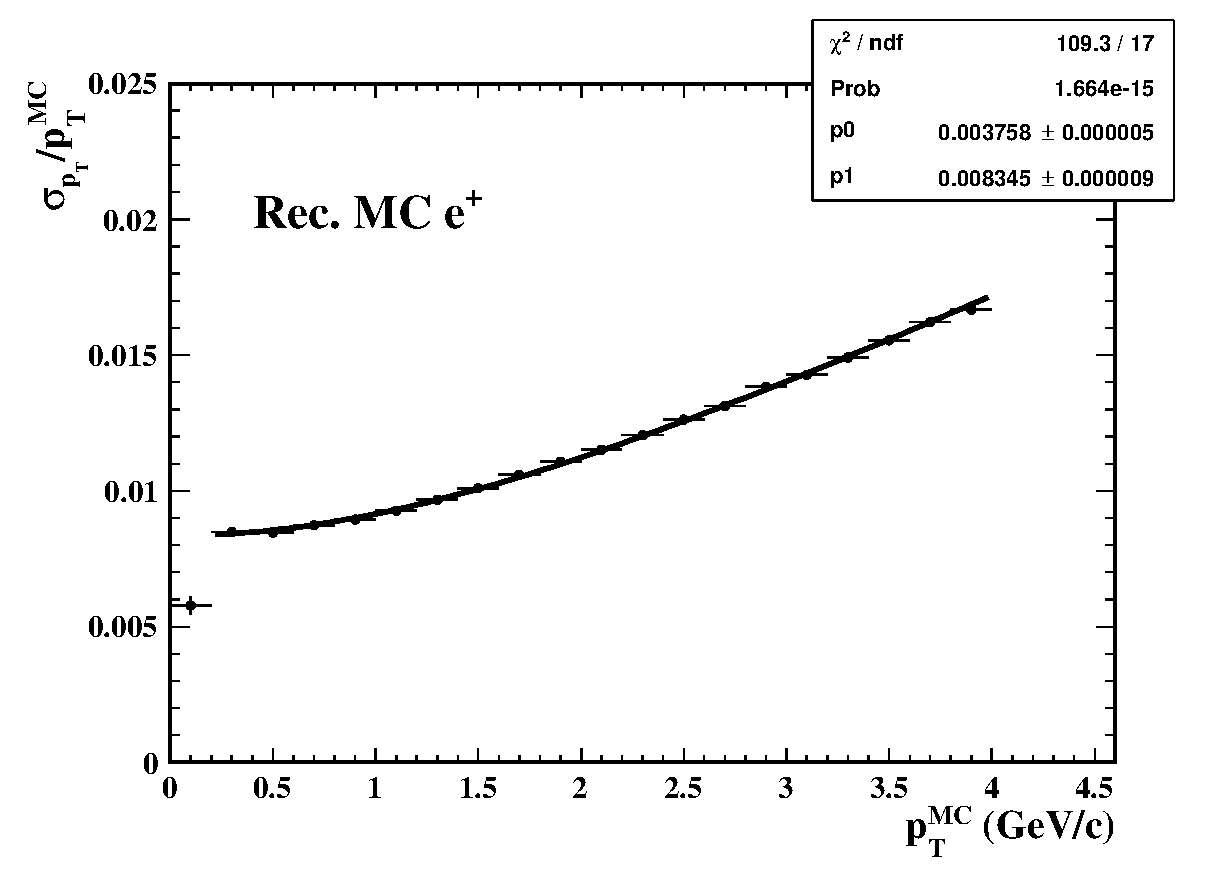
\includegraphics[keepaspectratio,width=0.6\textwidth]{analysis/positron_momRes.eps}
\figcaption{The transverse momentum resolution for positron as a function of $p_{T}$ from Run12 U + U minimum-bias embedding sample.}
 \label{ptres}
\end{figure}

Figure~\ref{uu193cock} shows the cocktail simulation within STAR acceptance including the light hadrons decay and correlated heavy flavor decay in U + U minimum-bias collisions at 193 GeV. The cocktails of different acceptance settings and the cocktail within STAR acceptance including the detector efficiency losses in U + U minimum-bias collisions at 193 GeV are depicted in Fig.~\ref{cocktails}. As discussed in Sec.~\ref{paireff}, the dielectron pair efficiency within STAR acceptance and STAR acceptance factor can be evaluated from Fig.~\ref{cocktails}.
\begin{figure}[htbp]
\begin{minipage}[htbp]{0.48\linewidth}
\centering
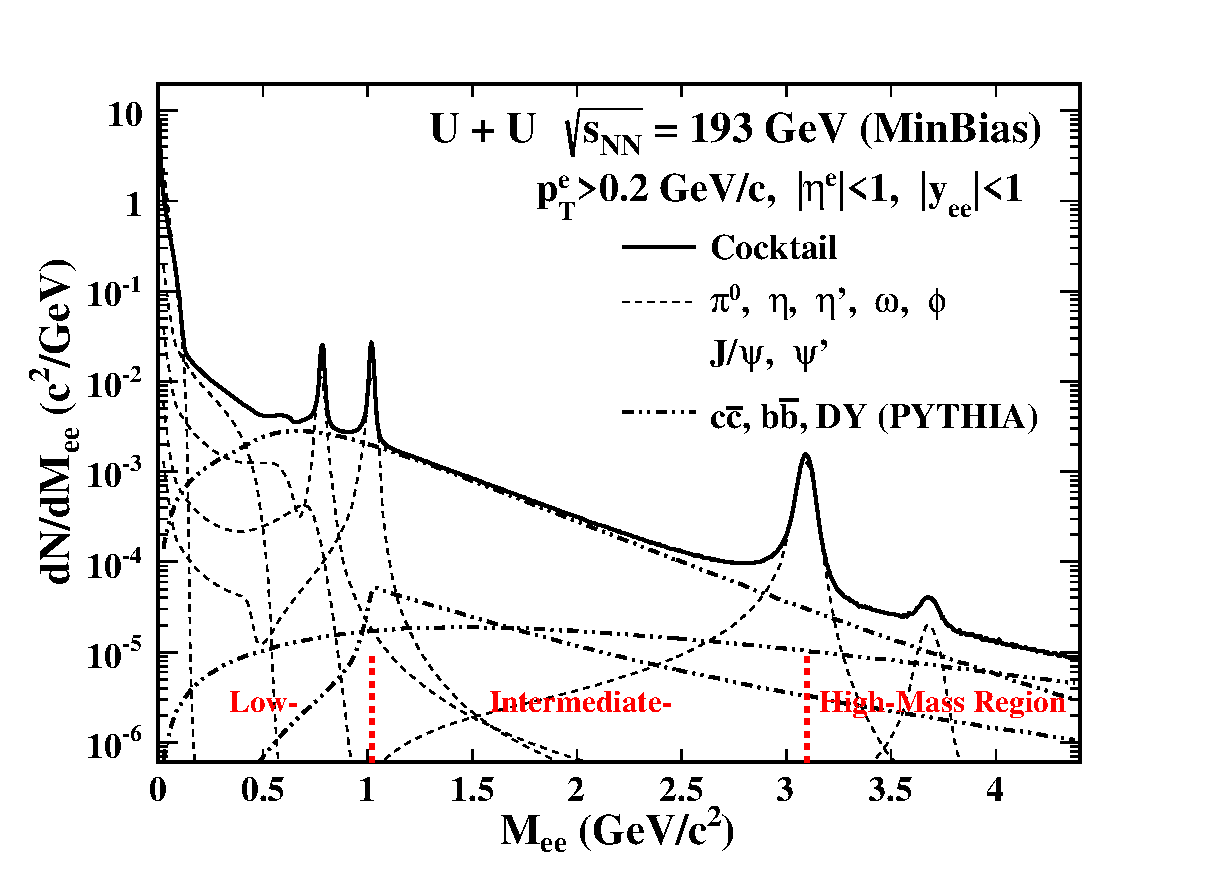
\includegraphics[width=1.0\textwidth]{analysis/UU193GeV_Cock.eps}
\caption{The cocktail simulation within STAR acceptance (solid line) including the light hadrons decay and correlated heavy flavor decay (dashed lines) in U + U minimum-bias collisions at 193 GeV.\label{uu193cock}}
\end{minipage}
\hfill
\begin{minipage}[htbp]{0.48\linewidth}
\centering
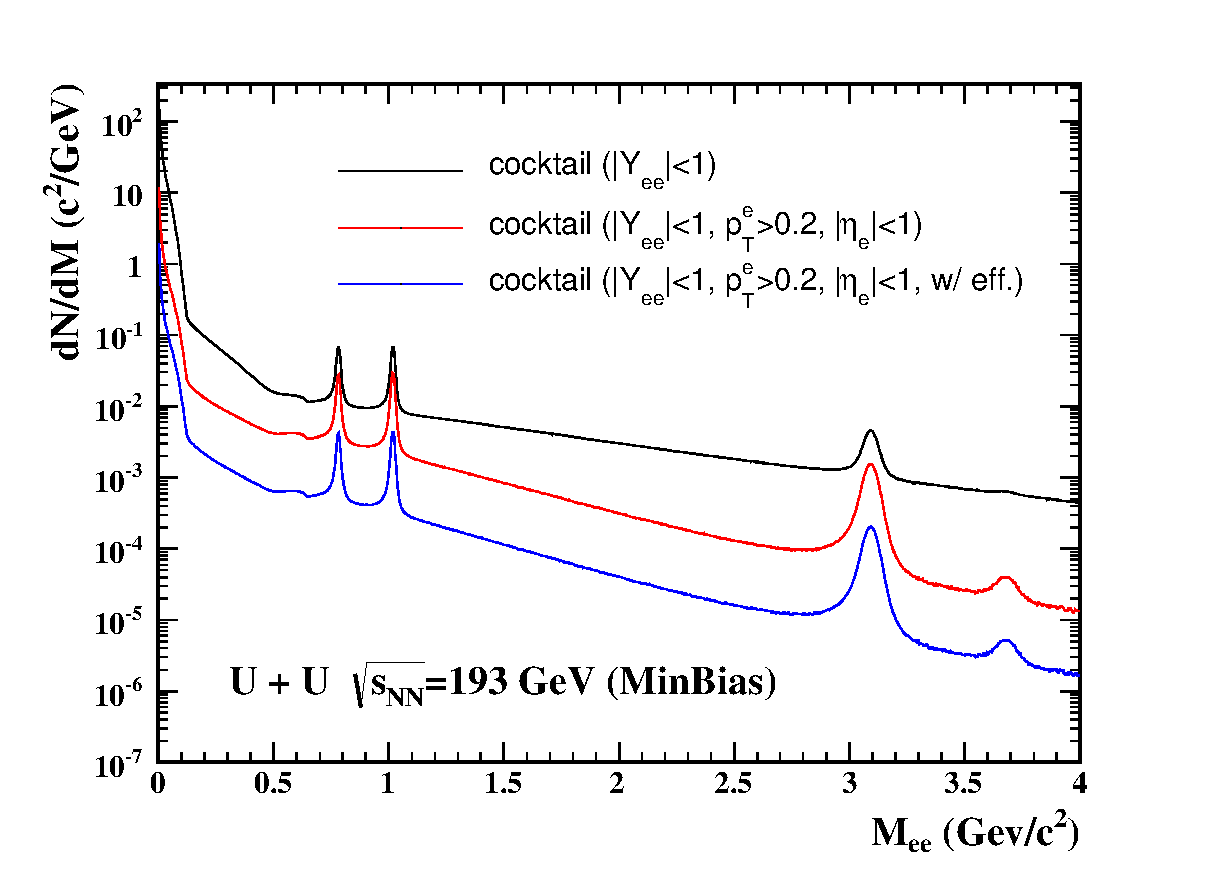
\includegraphics[width=1.0\textwidth]{analysis/minibias_cocktail.eps} 
\caption{The cocktails of different acceptance settings (Black - before filtering STAR acceptance; Red - within STAR acceptance) and the cocktail within STAR acceptance including the detector efficiency losses (Blue) in U + U minimum-bias collisions at 193 GeV.\label{cocktails}}
\end{minipage}
\end{figure}

\section{Systematic Uncertainties}
\label{sysUncertainty}

The sources of the systematic uncertainty that contribute to the final result in this analysis are listed below:
\begin{itemize}
\item[(i)] Background subtraction.
\item[(ii)] Hadron contamination. 
\item[(iii)] Efficiency correction.
\item[(iv)] Cocktail simulation.
\end{itemize} 

\paragraph{Background subtraction} In this analysis, the acceptance corrected like-sign background is subtracted for obtaining the raw signal. Where the acceptance factor is calculated by the the ratio of the mixed-event unlike-sign and like-sign distribution. The systematic uncertainty of the acceptance factor can be evaluated by varying the event categories (varying the number of  $V_{z}$, centrality and event-plane bins) and event-pool size. The difference between 2-D ($M_{ee}$, $p_{T}^{ee}$) and 1-D ($M_{ee}$) acceptance corrections is also taken into account.

\paragraph{Hadron contamination} The identified electron candidates contain a small amount of fast hadrons, as discussed in Sec.~\ref{purity}. If these hadrons are correlated with other particles (e.g. resonance decays), they may contribute into the final signal spectrum. The electron purity and the relative ratios of hadron over electron in the identified electron sample are shown in Fig.~\ref{electronpurity} and Fig.~\ref{hadroncon}, respectively. To estimate the contribution of the hadron contamination, the pure hadron samples are firstly selected by a tight $m^{2}$ cut (shown in Fig.~\ref{purehadron}). We randomly picked hadrons from these pure samples according to the hadron contamination levels in both total and the $p_{T}$ differential yields, creating a hadron pool. The same procedure used in the dielectron analysis is applied to the hadron contamination pool to estimate the $e-h$ and $h-h$ contribution. The effect in U + U collisions at 193 GeV should be similar to that in Au + Au collisions at 200 GeV. According to the published STAR dielectron long paper~\cite{STAR:dielectron1}, the relative contribution to the final spectrum is <5\% between 1 and 3 GeV/$c^{2}$.

\begin{figure}[htbp]
\begin{minipage}[htbp]{0.49\linewidth}
\centering
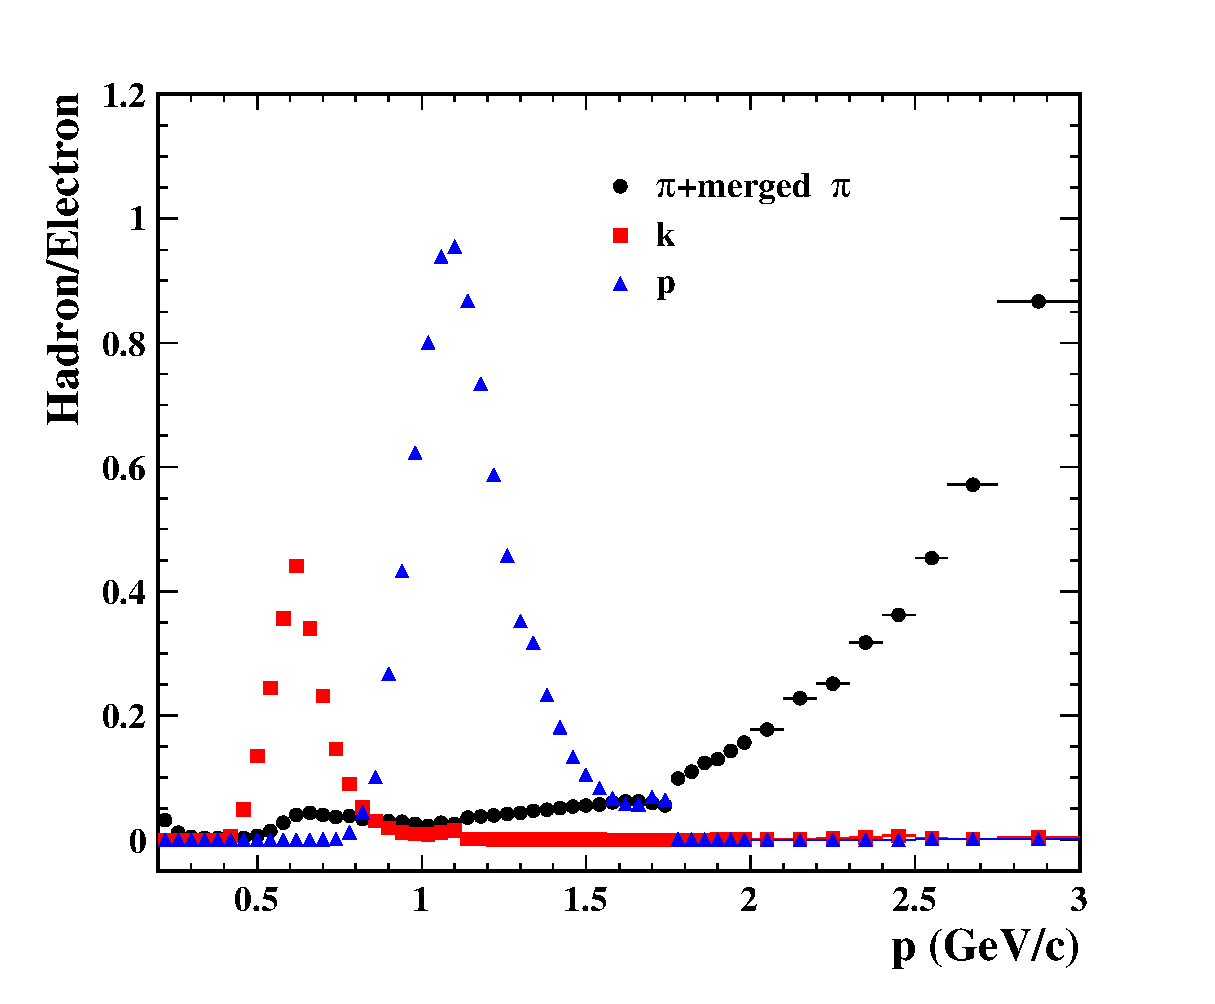
\includegraphics[width=1.0\textwidth]{analysis/hardon_contamination.eps}
\caption{The relative ratio of hadrons over electrons in the identified electron sample as a function of momentum.\label{hadroncon}}
\end{minipage}
\hfill
\begin{minipage}[htbp]{0.49\linewidth}
\centering
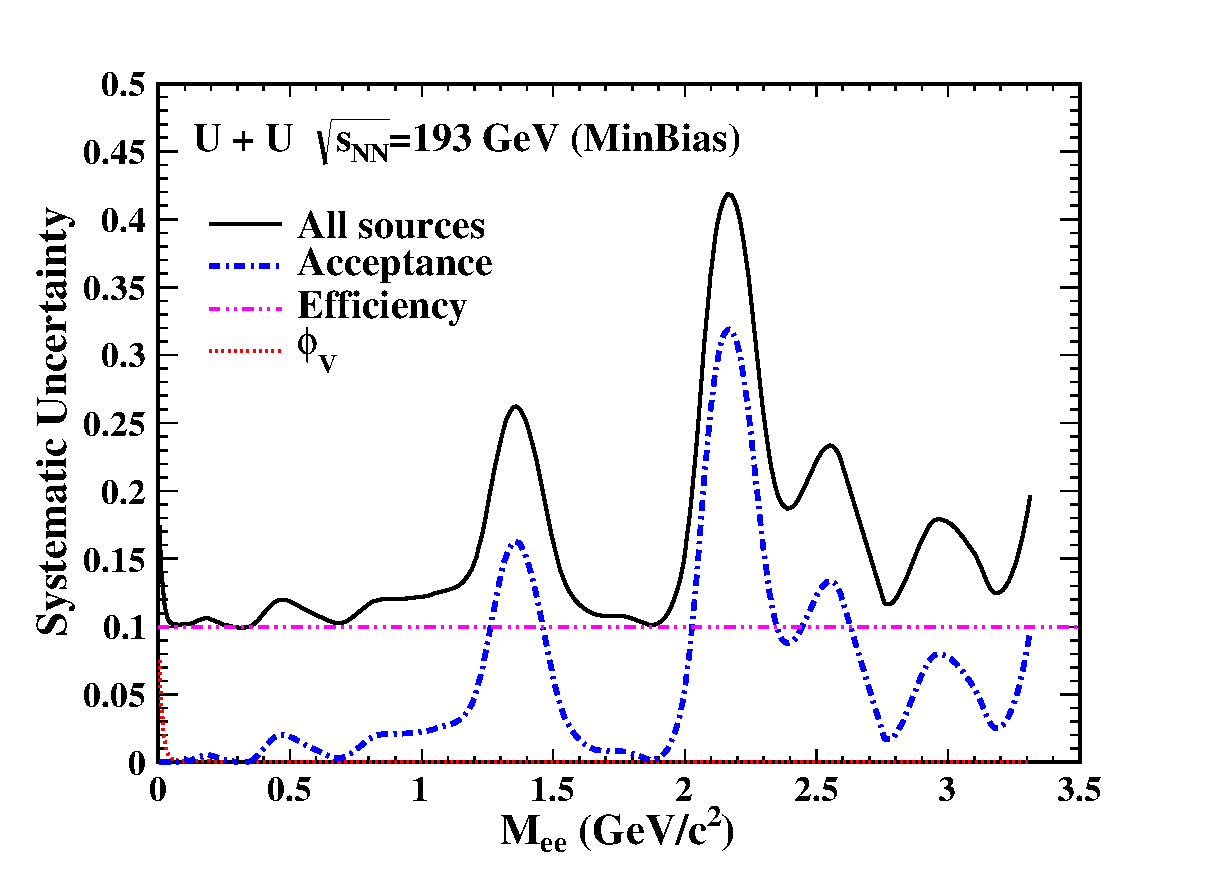
\includegraphics[width=1.0\textwidth]{analysis/Minibias_SysUncertainty.eps} 
\caption{The overall systematic uncertainty together with the major sources that contribute to the final result in U + U minimum-bias collisions at 193 GeV.\label{sysuncertainty}}
\end{minipage}
\end{figure}

\paragraph{Efficiency correction} The systematic uncertainty caused by efficiency correction includes uncertainties on the single track efficiency which is folded into the pair efficiency, the pair efficiency evaluated by different methods and the $\phi_{V}$ cut efficiency. The systematic uncertainty on TPC tracking efficiency (nHitsFit, dca) is evaluated by varying the selection cuts in the data and MC embedding at the same time and then comparing the difference between the change of data and MC embedding. The systematic uncertainties on nHitsDedx cut, $n\sigma_{e}$ cut and the TOF matching are evaluated by comparing the corresponding efficiency differences between different pure electron samples (using different invariant mass cuts to select the pure electron samples). The systematic uncertainty on the $1/\beta$ cut efficiency is evaluated by comparing the efficiency difference between direct bin counting method and Gaussian fit (discussed in Sec.~\ref{eideff}). These systematic uncertainties owing to the single track efficiency are summarized in Tab.~\ref{singletrkeffuncertainty}. Due to the unknown heavy flavor correlation in the medium, two extreme methods (discussed in Sec.~\ref{paireff}) are employed to fold the single track efficiency into the pair efficiency. The difference of the pair efficiency between these two methods are also taken into account for the efficiency correction systematic uncertainty. The systematic uncertainty of the $\phi_{V}$ cut efficiency is evaluated by comparing the difference between the efficiency from the $\pi^{0}$ embedding sample and the virtual photon decay sample.

\paragraph{Cocktail simulation}  The systematic uncertainty of the cocktail simulation is evaluated by folding the systematic uncertainties of meson yields and the heavy flavor cross sections.

 The systematic uncertainties of the final dielectron invariant mass spectra are summarized in Fig.~\ref{sysuncertainty}. The total systematic uncertainty, shown in Fig.~\ref{sysuncertainty}, is obtained by a direct sum of the contribution of each individual component listed at the beginning of this section. 

\begin{table}[htp]
\centering
\caption{Systematic uncertainties on single track efficiency.}
\label{singletrkeffuncertainty}
\newcolumntype{V}{!{\vrule width 1.6pt}}
\begin{tabular}{ccc}
\Xhline{1.6pt}
 & Component & Uncertainty (\%) \\
\Xhline{1.2pt}
\multirow{4}*{TPC} & nHitsFit & 3.4\\ 
& DCA & 1.8 \\
& nHitsdEdx & 1.1 \\
& n$\sigma_{e}$ & 0.5 \\ 
\Xhline{1.2pt}
 \multirow{2}*{TOF} & Matching & 1.4 \\
 & $1/\beta$ & 2.4 \\
 \Xhline{1.2pt}
 Total && 4.9 \\
\Xhline{1.6pt}
\end{tabular}
\end{table}
